\documentclass[]{article}
\usepackage{lmodern}
\usepackage{amssymb,amsmath}
\usepackage{ifxetex,ifluatex}
\usepackage{fixltx2e} % provides \textsubscript
\ifnum 0\ifxetex 1\fi\ifluatex 1\fi=0 % if pdftex
  \usepackage[T1]{fontenc}
  \usepackage[utf8]{inputenc}
\else % if luatex or xelatex
  \ifxetex
    \usepackage{mathspec}
  \else
    \usepackage{fontspec}
  \fi
  \defaultfontfeatures{Ligatures=TeX,Scale=MatchLowercase}
\fi
% use upquote if available, for straight quotes in verbatim environments
\IfFileExists{upquote.sty}{\usepackage{upquote}}{}
% use microtype if available
\IfFileExists{microtype.sty}{%
\usepackage{microtype}
\UseMicrotypeSet[protrusion]{basicmath} % disable protrusion for tt fonts
}{}
\usepackage[margin=1in]{geometry}
\usepackage{hyperref}
\hypersetup{unicode=true,
            pdftitle={Modern Data Mining - HW 3},
            pdfauthor={Anirudh Bajaj; Esther Shin; Matt LeBaron; Raman Chadha},
            pdfborder={0 0 0},
            breaklinks=true}
\urlstyle{same}  % don't use monospace font for urls
\usepackage{color}
\usepackage{fancyvrb}
\newcommand{\VerbBar}{|}
\newcommand{\VERB}{\Verb[commandchars=\\\{\}]}
\DefineVerbatimEnvironment{Highlighting}{Verbatim}{commandchars=\\\{\}}
% Add ',fontsize=\small' for more characters per line
\usepackage{framed}
\definecolor{shadecolor}{RGB}{248,248,248}
\newenvironment{Shaded}{\begin{snugshade}}{\end{snugshade}}
\newcommand{\KeywordTok}[1]{\textcolor[rgb]{0.13,0.29,0.53}{\textbf{#1}}}
\newcommand{\DataTypeTok}[1]{\textcolor[rgb]{0.13,0.29,0.53}{#1}}
\newcommand{\DecValTok}[1]{\textcolor[rgb]{0.00,0.00,0.81}{#1}}
\newcommand{\BaseNTok}[1]{\textcolor[rgb]{0.00,0.00,0.81}{#1}}
\newcommand{\FloatTok}[1]{\textcolor[rgb]{0.00,0.00,0.81}{#1}}
\newcommand{\ConstantTok}[1]{\textcolor[rgb]{0.00,0.00,0.00}{#1}}
\newcommand{\CharTok}[1]{\textcolor[rgb]{0.31,0.60,0.02}{#1}}
\newcommand{\SpecialCharTok}[1]{\textcolor[rgb]{0.00,0.00,0.00}{#1}}
\newcommand{\StringTok}[1]{\textcolor[rgb]{0.31,0.60,0.02}{#1}}
\newcommand{\VerbatimStringTok}[1]{\textcolor[rgb]{0.31,0.60,0.02}{#1}}
\newcommand{\SpecialStringTok}[1]{\textcolor[rgb]{0.31,0.60,0.02}{#1}}
\newcommand{\ImportTok}[1]{#1}
\newcommand{\CommentTok}[1]{\textcolor[rgb]{0.56,0.35,0.01}{\textit{#1}}}
\newcommand{\DocumentationTok}[1]{\textcolor[rgb]{0.56,0.35,0.01}{\textbf{\textit{#1}}}}
\newcommand{\AnnotationTok}[1]{\textcolor[rgb]{0.56,0.35,0.01}{\textbf{\textit{#1}}}}
\newcommand{\CommentVarTok}[1]{\textcolor[rgb]{0.56,0.35,0.01}{\textbf{\textit{#1}}}}
\newcommand{\OtherTok}[1]{\textcolor[rgb]{0.56,0.35,0.01}{#1}}
\newcommand{\FunctionTok}[1]{\textcolor[rgb]{0.00,0.00,0.00}{#1}}
\newcommand{\VariableTok}[1]{\textcolor[rgb]{0.00,0.00,0.00}{#1}}
\newcommand{\ControlFlowTok}[1]{\textcolor[rgb]{0.13,0.29,0.53}{\textbf{#1}}}
\newcommand{\OperatorTok}[1]{\textcolor[rgb]{0.81,0.36,0.00}{\textbf{#1}}}
\newcommand{\BuiltInTok}[1]{#1}
\newcommand{\ExtensionTok}[1]{#1}
\newcommand{\PreprocessorTok}[1]{\textcolor[rgb]{0.56,0.35,0.01}{\textit{#1}}}
\newcommand{\AttributeTok}[1]{\textcolor[rgb]{0.77,0.63,0.00}{#1}}
\newcommand{\RegionMarkerTok}[1]{#1}
\newcommand{\InformationTok}[1]{\textcolor[rgb]{0.56,0.35,0.01}{\textbf{\textit{#1}}}}
\newcommand{\WarningTok}[1]{\textcolor[rgb]{0.56,0.35,0.01}{\textbf{\textit{#1}}}}
\newcommand{\AlertTok}[1]{\textcolor[rgb]{0.94,0.16,0.16}{#1}}
\newcommand{\ErrorTok}[1]{\textcolor[rgb]{0.64,0.00,0.00}{\textbf{#1}}}
\newcommand{\NormalTok}[1]{#1}
\usepackage{graphicx,grffile}
\makeatletter
\def\maxwidth{\ifdim\Gin@nat@width>\linewidth\linewidth\else\Gin@nat@width\fi}
\def\maxheight{\ifdim\Gin@nat@height>\textheight\textheight\else\Gin@nat@height\fi}
\makeatother
% Scale images if necessary, so that they will not overflow the page
% margins by default, and it is still possible to overwrite the defaults
% using explicit options in \includegraphics[width, height, ...]{}
\setkeys{Gin}{width=\maxwidth,height=\maxheight,keepaspectratio}
\IfFileExists{parskip.sty}{%
\usepackage{parskip}
}{% else
\setlength{\parindent}{0pt}
\setlength{\parskip}{6pt plus 2pt minus 1pt}
}
\setlength{\emergencystretch}{3em}  % prevent overfull lines
\providecommand{\tightlist}{%
  \setlength{\itemsep}{0pt}\setlength{\parskip}{0pt}}
\setcounter{secnumdepth}{0}
% Redefines (sub)paragraphs to behave more like sections
\ifx\paragraph\undefined\else
\let\oldparagraph\paragraph
\renewcommand{\paragraph}[1]{\oldparagraph{#1}\mbox{}}
\fi
\ifx\subparagraph\undefined\else
\let\oldsubparagraph\subparagraph
\renewcommand{\subparagraph}[1]{\oldsubparagraph{#1}\mbox{}}
\fi

%%% Use protect on footnotes to avoid problems with footnotes in titles
\let\rmarkdownfootnote\footnote%
\def\footnote{\protect\rmarkdownfootnote}

%%% Change title format to be more compact
\usepackage{titling}

% Create subtitle command for use in maketitle
\newcommand{\subtitle}[1]{
  \posttitle{
    \begin{center}\large#1\end{center}
    }
}

\setlength{\droptitle}{-2em}

  \title{Modern Data Mining - HW 3}
    \pretitle{\vspace{\droptitle}\centering\huge}
  \posttitle{\par}
    \author{Anirudh Bajaj \\ Esther Shin \\ Matt LeBaron \\ Raman Chadha}
    \preauthor{\centering\large\emph}
  \postauthor{\par}
    \date{}
    \predate{}\postdate{}
  

\begin{document}
\maketitle

\begin{Shaded}
\begin{Highlighting}[]
\NormalTok{knitr}\OperatorTok{::}\NormalTok{opts_chunk}\OperatorTok{$}\KeywordTok{set}\NormalTok{(}\DataTypeTok{fig.height=}\DecValTok{4}\NormalTok{, }\DataTypeTok{fig.width=}\DecValTok{6}\NormalTok{, }\DataTypeTok{warning =}\NormalTok{ F)}

\CommentTok{# constants for homework assignments}
\NormalTok{hw_num <-}\StringTok{ }\DecValTok{3}
\NormalTok{hw_due_date <-}\StringTok{ "28 October, 2018"}
\end{Highlighting}
\end{Shaded}

\subsection{Overview / Instructions}\label{overview-instructions}

This is homework \#3 of STAT 471/571/701. It will be \textbf{due on 28
October, 2018 by 11:59 PM} on Canvas. You can directly edit this file to
add your answers. Submit the Rmd file, a PDF or word or HTML version
with \textbf{only 1 submission} per HW team.

\textbf{Note:} To minimize your work and errors, we provide this Rmd
file to guide you in the process of building your final report. To that
end, we've included code to load the necessary data files. Make sure
that the following files are in the same folder as this R Markdown file:

\begin{itemize}
\tightlist
\item
  \texttt{FRAMINGHAM.dat}
\item
  \texttt{Bills.subset.csv}
\item
  \texttt{Bills.subset.test.csv}
\end{itemize}

The data should load properly if you are working in Rstudio,
\emph{without needing to change your working directory}.

Solutions will be posted. Make sure to compare your answers to and
understand the solutions.

\subsection{R Markdown / Knitr tips}\label{r-markdown-knitr-tips}

You should think of this R Markdown file as generating a polished
report, one that you would be happy to show other people (or your boss).
There shouldn't be any extraneous output; all graphs and code run should
clearly have a reason to be run. That means that any output in the final
file should have explanations.

A few tips:

\begin{itemize}
\tightlist
\item
  Keep each chunk to only output one thing! In R, if you're not doing an
  assignment (with the \texttt{\textless{}-} operator), it's probably
  going to print something.
\item
  If you don't want to print the R code you wrote (but want to run it,
  and want to show the results), use a chunk declaration like this:
  \texttt{\{r,\ echo=F\}}
\item
  If you don't want to show the results of the R code or the original
  code, use a chunk declaration like: \texttt{\{r,\ include=F\}}
\item
  If you don't want to show the results, but show the original code, use
  a chunk declaration like:
  \texttt{\{r,\ results=\textquotesingle{}hide\textquotesingle{}\}}.
\item
  If you don't want to run the R code at all use
  \texttt{\{r,\ eval\ =\ F\}}.
\item
  We show a few examples of these options in the below example code.
\item
  For more details about these R Markdown options, see the
  \href{http://yihui.name/knitr/options/}{documentation}.
\item
  Delete the instructions and this R Markdown section, since they're not
  part of your overall report.
\end{itemize}

\subsection{Problem 0}\label{problem-0}

Review the code and concepts covered during lecture, in particular,
logistic regression and classification.

\subsection{Problem 1}\label{problem-1}

We will continue to use the Framingham Data (\texttt{Framingham.dat}) so
that you are already familiar with the data and the variables. All the
results are obtained through training data.

To keep our answers consistent, use a subset of the data, and exclude
anyone with a missing entry. For your convenience, we've loaded it here
together with a brief summary about the data.

We note that this dataset contains 311 people diagnosed with heart
disease and 1095 without heart disease.

\begin{verbatim}
  
     0    1 
  1095  311
\end{verbatim}

After a quick cleaning up here is a summary about the data:

\begin{Shaded}
\begin{Highlighting}[]
\CommentTok{# using the comment="     ", we get rid of the ## in the output.}
\KeywordTok{summary}\NormalTok{(hd_data.f)}
\end{Highlighting}
\end{Shaded}

\begin{verbatim}
       HD            AGE            SEX           SBP             DBP        
       0:1086   Min.   :45.00   FEMALE:730   Min.   : 90.0   Min.   : 50.00  
       1: 307   1st Qu.:48.00   MALE  :663   1st Qu.:130.0   1st Qu.: 80.00  
                Median :52.00                Median :142.0   Median : 90.00  
                Mean   :52.43                Mean   :148.1   Mean   : 90.16  
                3rd Qu.:56.00                3rd Qu.:160.0   3rd Qu.: 98.00  
                Max.   :62.00                Max.   :300.0   Max.   :160.00  
            CHOL            FRW             CIG        
       Min.   : 96.0   Min.   : 52.0   Min.   : 0.000  
       1st Qu.:200.0   1st Qu.: 94.0   1st Qu.: 0.000  
       Median :230.0   Median :103.0   Median : 0.000  
       Mean   :234.6   Mean   :105.4   Mean   : 8.035  
       3rd Qu.:264.0   3rd Qu.:114.0   3rd Qu.:20.000  
       Max.   :430.0   Max.   :222.0   Max.   :60.000
\end{verbatim}

\subsubsection{Part 1A}\label{part-1a}

Conceptual questions to understand building blocks of logistic
regression. All the codes in this part should be hidden.

\begin{enumerate}
\def\labelenumi{\roman{enumi}.}
\tightlist
\item
  Take a random subsample of size 5 from \texttt{hd\_data\_f} which only
  includes \texttt{HD} and \texttt{SBP}. Also set \texttt{set.seed(50)}.
  List the three observations neatly below. No code should be shown
  here.
\end{enumerate}

\begin{verbatim}
##      HD SBP
## 996   0 142
## 614   0 126
## 281   0 136
## 1075  0 178
## 719   0 126
\end{verbatim}

\begin{enumerate}
\def\labelenumi{\roman{enumi}.}
\setcounter{enumi}{1}
\tightlist
\item
  Write down the likelihood function using the five observations above.
\end{enumerate}

\[\begin{split}
\mathcal{Lik}(\beta_0, \beta_1 \vert {\text Data}) &= {\text {Prob(the outcome of the data)}}\\
&=Prob((Y=0|SBP=142), (Y=0|SBP=126), (Y=0|SBP=136), (Y=0|SBP=178), (Y=0|SBP=126)) \\
&=Prob(Y=0|SBP=142) \times Prob(Y=0|SBP=126) \times Prob(Y=0|SBP=136) \times Prob(Y=0|SBP=178) \times Prob(Y=0|SBP=126)) \\
&= \frac{1}{1+e^{\beta_0 + 142 \beta_1}}\cdot\frac{1}{1+e^{\beta_0 + 126\beta_1}}\cdot\frac{1}{1 + e^{\beta_0 + 136 \beta_1}}\cdot\frac{1}{1 + e^{\beta_0 + 178 \beta_1}}\cdot\frac{1}{1 + e^{\beta_0 + 126 \beta_1}}
    \end{split}\]

\begin{enumerate}
\def\labelenumi{\roman{enumi}.}
\setcounter{enumi}{2}
\tightlist
\item
  Find the MLE's based on this subset. Report the estimated logit
  function and the probability of \texttt{HD}=1. Briefly explain how the
  MLE's are obtained based on ii. above.
\end{enumerate}

\begin{Shaded}
\begin{Highlighting}[]
\NormalTok{mle.sample <-}\StringTok{ }\KeywordTok{glm}\NormalTok{(HD}\OperatorTok{~}\NormalTok{SBP, sample.data, }\DataTypeTok{family=}\KeywordTok{binomial}\NormalTok{(logit))}
\KeywordTok{summary}\NormalTok{(mle.sample)}
\end{Highlighting}
\end{Shaded}

\begin{verbatim}
## 
## Call:
## glm(formula = HD ~ SBP, family = binomial(logit), data = sample.data)
## 
## Deviance Residuals: 
##        996         614         281        1075         719  
## -6.547e-06  -6.547e-06  -6.547e-06  -6.547e-06  -6.547e-06  
## 
## Coefficients:
##              Estimate Std. Error z value Pr(>|z|)
## (Intercept)    -24.57  436053.61       0        1
## SBP              0.00    3051.55       0        1
## 
## (Dispersion parameter for binomial family taken to be 1)
## 
##     Null deviance: 0.0000e+00  on 4  degrees of freedom
## Residual deviance: 2.1434e-10  on 3  degrees of freedom
## AIC: 4
## 
## Number of Fisher Scoring iterations: 23
\end{verbatim}

Probability function estimated by glm using only the above 5 sample
observations:

logit = -24.57 + 0.00 SBP

\(P(HD = 1 \vert SBP) = \frac{e^{-24.57+0.00 \times SBP}}{1+e^{-24.57+0.00 \times SBP}}\)

\begin{Shaded}
\begin{Highlighting}[]
\CommentTok{#calculated probability}
\KeywordTok{exp}\NormalTok{(}\OperatorTok{-}\FloatTok{24.57}\NormalTok{)}\OperatorTok{/}\NormalTok{\{}\DecValTok{1}\OperatorTok{+}\KeywordTok{exp}\NormalTok{(}\OperatorTok{-}\FloatTok{24.57}\NormalTok{)\}}
\end{Highlighting}
\end{Shaded}

\begin{verbatim}
## [1] 2.134935e-11
\end{verbatim}

\section{MLE is the maximul likelihood of observing the predicted data,
given the input data. Mathematically, taking log both sides of the
equation and differentiating it and equating to 0 leads to the logit
function. GLM iterates on Beta0 and Beta1 values to maximize this
probability. In the above case, the probability of HD=1 is very low.
This is because the input sample data does not have any patient with
heart disease. The SBP slope is 0, but also note that the intercept and
SBP values are independently both not
singnificant.}\label{mle-is-the-maximul-likelihood-of-observing-the-predicted-data-given-the-input-data.-mathematically-taking-log-both-sides-of-the-equation-and-differentiating-it-and-equating-to-0-leads-to-the-logit-function.-glm-iterates-on-beta0-and-beta1-values-to-maximize-this-probability.-in-the-above-case-the-probability-of-hd1-is-very-low.-this-is-because-the-input-sample-data-does-not-have-any-patient-with-heart-disease.-the-sbp-slope-is-0-but-also-note-that-the-intercept-and-sbp-values-are-independently-both-not-singnificant.}

\subsubsection{Part 1B}\label{part-1b}

Goal: Identify important risk factors for \texttt{Heart.Disease.}
through logistic regression. Start a fit with just one factor,
\texttt{SBP}, and call it \texttt{fit1}. Let us add one variable to this
at a time from among the rest of the variables.

\begin{Shaded}
\begin{Highlighting}[]
\NormalTok{fit1 <-}\StringTok{ }\KeywordTok{glm}\NormalTok{(HD}\OperatorTok{~}\NormalTok{SBP, hd_data.f, }\DataTypeTok{family=}\NormalTok{binomial)}
\KeywordTok{summary}\NormalTok{(fit1)}
\NormalTok{fit1.}\DecValTok{1}\NormalTok{ <-}\StringTok{ }\KeywordTok{glm}\NormalTok{(HD}\OperatorTok{~}\NormalTok{SBP }\OperatorTok{+}\StringTok{ }\NormalTok{AGE, hd_data.f, }\DataTypeTok{family=}\NormalTok{binomial)}
\KeywordTok{summary}\NormalTok{(fit1.}\DecValTok{1}\NormalTok{)}
\NormalTok{fit1.}\DecValTok{2}\NormalTok{ <-}\StringTok{ }\KeywordTok{glm}\NormalTok{(HD}\OperatorTok{~}\NormalTok{SBP }\OperatorTok{+}\StringTok{ }\NormalTok{SEX, hd_data.f, }\DataTypeTok{family=}\NormalTok{binomial)}
\KeywordTok{summary}\NormalTok{(fit1.}\DecValTok{2}\NormalTok{)}
\NormalTok{fit1.}\DecValTok{3}\NormalTok{ <-}\StringTok{ }\KeywordTok{glm}\NormalTok{(HD}\OperatorTok{~}\NormalTok{SBP }\OperatorTok{+}\StringTok{ }\NormalTok{DBP, hd_data.f, }\DataTypeTok{family=}\NormalTok{binomial)}
\KeywordTok{summary}\NormalTok{(fit1.}\DecValTok{3}\NormalTok{)}
\NormalTok{fit1.}\DecValTok{4}\NormalTok{ <-}\StringTok{ }\KeywordTok{glm}\NormalTok{(HD}\OperatorTok{~}\NormalTok{SBP }\OperatorTok{+}\StringTok{ }\NormalTok{CHOL, hd_data.f, }\DataTypeTok{family=}\NormalTok{binomial)}
\KeywordTok{summary}\NormalTok{(fit1.}\DecValTok{4}\NormalTok{)}
\NormalTok{fit1.}\DecValTok{5}\NormalTok{ <-}\StringTok{ }\KeywordTok{glm}\NormalTok{(HD}\OperatorTok{~}\NormalTok{SBP }\OperatorTok{+}\StringTok{ }\NormalTok{DBP, hd_data.f, }\DataTypeTok{family=}\NormalTok{binomial)}
\KeywordTok{summary}\NormalTok{(fit1.}\DecValTok{5}\NormalTok{)}
\NormalTok{fit1.}\DecValTok{6}\NormalTok{ <-}\StringTok{ }\KeywordTok{glm}\NormalTok{(HD}\OperatorTok{~}\NormalTok{SBP }\OperatorTok{+}\StringTok{ }\NormalTok{FRW, hd_data.f, }\DataTypeTok{family=}\NormalTok{binomial)}
\KeywordTok{summary}\NormalTok{(fit1.}\DecValTok{6}\NormalTok{)}
\NormalTok{fit1.}\DecValTok{7}\NormalTok{ <-}\StringTok{ }\KeywordTok{glm}\NormalTok{(HD}\OperatorTok{~}\NormalTok{SBP }\OperatorTok{+}\StringTok{ }\NormalTok{CIG, hd_data.f, }\DataTypeTok{family=}\NormalTok{binomial)}
\KeywordTok{summary}\NormalTok{(fit1.}\DecValTok{7}\NormalTok{)}
\end{Highlighting}
\end{Shaded}

\begin{enumerate}
\def\labelenumi{\roman{enumi}.}
\tightlist
\item
  Which single variable would be the most important to add? Add it to
  your model, and call the new fit \texttt{fit2}.
\end{enumerate}

\begin{Shaded}
\begin{Highlighting}[]
\CommentTok{#Based on AIC values (lowest is best), Sex is the most important variable to add. Adding it to the model:}
\NormalTok{fit2 <-}\StringTok{ }\KeywordTok{glm}\NormalTok{(HD}\OperatorTok{~}\NormalTok{SBP }\OperatorTok{+}\StringTok{ }\NormalTok{SEX, hd_data.f, }\DataTypeTok{family=}\NormalTok{binomial)}
\KeywordTok{summary}\NormalTok{(fit2)}
\end{Highlighting}
\end{Shaded}

\begin{verbatim}
## 
## Call:
## glm(formula = HD ~ SBP + SEX, family = binomial, data = hd_data.f)
## 
## Deviance Residuals: 
##     Min       1Q   Median       3Q      Max  
## -1.6408  -0.7373  -0.5726  -0.4169   2.2452  
## 
## Coefficients:
##              Estimate Std. Error z value Pr(>|z|)    
## (Intercept) -4.570256   0.389727 -11.727  < 2e-16 ***
## SBP          0.018717   0.002324   8.053 8.07e-16 ***
## SEXMALE      0.903420   0.139762   6.464 1.02e-10 ***
## ---
## Signif. codes:  0 '***' 0.001 '**' 0.01 '*' 0.05 '.' 0.1 ' ' 1
## 
## (Dispersion parameter for binomial family taken to be 1)
## 
##     Null deviance: 1469.3  on 1392  degrees of freedom
## Residual deviance: 1373.8  on 1390  degrees of freedom
## AIC: 1379.8
## 
## Number of Fisher Scoring iterations: 4
\end{verbatim}

We will pick up the variable either with highest \(|z|\) value, or
smallest \(p\) value. From all the two variable models we see that
\texttt{SEX} will be the most important addition on top of the SBP. And
here is the summary report.

\begin{Shaded}
\begin{Highlighting}[]
\NormalTok{## How to control the summary(fit2) output to cut some junk?}
\NormalTok{## We could use packages: xtable or broom. }
\KeywordTok{library}\NormalTok{(xtable)}
\KeywordTok{options}\NormalTok{(}\DataTypeTok{xtable.comment =} \OtherTok{FALSE}\NormalTok{)}
\NormalTok{fit2 <-}\StringTok{ }\KeywordTok{glm}\NormalTok{(HD}\OperatorTok{~}\NormalTok{SBP }\OperatorTok{+}\StringTok{ }\NormalTok{SEX, hd_data.f, }\DataTypeTok{family=}\NormalTok{binomial)}
\KeywordTok{xtable}\NormalTok{(fit2)}
\end{Highlighting}
\end{Shaded}

\begin{verbatim}
## \begin{table}[ht]
## \centering
## \begin{tabular}{rrrrr}
##   \hline
##  & Estimate & Std. Error & z value & Pr($>$$|$z$|$) \\ 
##   \hline
## (Intercept) & -4.5703 & 0.3897 & -11.73 & 0.0000 \\ 
##   SBP & 0.0187 & 0.0023 & 8.05 & 0.0000 \\ 
##   SEXMALE & 0.9034 & 0.1398 & 6.46 & 0.0000 \\ 
##    \hline
## \end{tabular}
## \end{table}
\end{verbatim}

\begin{enumerate}
\def\labelenumi{\roman{enumi}.}
\setcounter{enumi}{1}
\tightlist
\item
  Is the residual deviance of \texttt{fit2} always smaller than that of
  \texttt{fit1}? Why or why not?
\end{enumerate}

\section{In fit2, we find that SEX is a significant variable (p-value
\textless{} 0.05), that is, controllig for SBP, we reject the null
hypothesis that SEX has no influence on the HD value. Whenever we add an
additional variable that is significant, the residual deviance will
always
decrease.}\label{in-fit2-we-find-that-sex-is-a-significant-variable-p-value-0.05-that-is-controllig-for-sbp-we-reject-the-null-hypothesis-that-sex-has-no-influence-on-the-hd-value.-whenever-we-add-an-additional-variable-that-is-significant-the-residual-deviance-will-always-decrease.}

\begin{enumerate}
\def\labelenumi{\roman{enumi}.}
\setcounter{enumi}{2}
\tightlist
\item
  Perform both the Wald test and the Likelihood ratio tests
  (Chi-Squared) to see if the added variable is significant at the .01
  level. What are the p-values from each test? Are they the same?
\end{enumerate}

\section{Likelihood Ratio test}\label{likelihood-ratio-test}

Null Deviance = 1469.3 Residual Deviance = 1373.8

\begin{Shaded}
\begin{Highlighting}[]
\NormalTok{chi_sq <-}\StringTok{ }\FloatTok{1469.3} \OperatorTok{-}\StringTok{ }\FloatTok{1373.8}
\KeywordTok{pchisq}\NormalTok{(chi_sq, }\DecValTok{1}\NormalTok{, }\DataTypeTok{lower.tail=}\OtherTok{FALSE}\NormalTok{)}
\end{Highlighting}
\end{Shaded}

\begin{verbatim}
## [1] 1.478913e-22
\end{verbatim}

\section{\texorpdfstring{Wald test (installing package ``survey'' to
directly conduct Wald
test)}{Wald test (installing package survey to directly conduct Wald test)}}\label{wald-test-installing-package-survey-to-directly-conduct-wald-test}

\begin{Shaded}
\begin{Highlighting}[]
\KeywordTok{library}\NormalTok{(survey)}
\end{Highlighting}
\end{Shaded}

\begin{verbatim}
## Loading required package: grid
\end{verbatim}

\begin{verbatim}
## Loading required package: Matrix
\end{verbatim}

\begin{verbatim}
## Loading required package: survival
\end{verbatim}

\begin{verbatim}
## 
## Attaching package: 'survey'
\end{verbatim}

\begin{verbatim}
## The following object is masked from 'package:graphics':
## 
##     dotchart
\end{verbatim}

\begin{Shaded}
\begin{Highlighting}[]
\KeywordTok{regTermTest}\NormalTok{(fit2, }\StringTok{"SEX"}\NormalTok{)}
\end{Highlighting}
\end{Shaded}

\begin{verbatim}
## Wald test for SEX
##  in glm(formula = HD ~ SBP + SEX, family = binomial, data = hd_data.f)
## F =  41.78308  on  1  and  1390  df: p= 1.4079e-10
\end{verbatim}

\section{The added variable SEX is significant at the 0.01 level.
p-value from Likelihood-Ratio test is 1.478913e-22 and from Wald test is
1.4079e-10. The p-values are different. Whereas Wald Test tests
significance of an individual variable (in this case SEX), Likelihood
Test tests significance of a set of variables (in this case SBP and
SEX).}\label{the-added-variable-sex-is-significant-at-the-0.01-level.-p-value-from-likelihood-ratio-test-is-1.478913e-22-and-from-wald-test-is-1.4079e-10.-the-p-values-are-different.-whereas-wald-test-tests-significance-of-an-individual-variable-in-this-case-sex-likelihood-test-tests-significance-of-a-set-of-variables-in-this-case-sbp-and-sex.}

\subsubsection{Part 1C - Model building}\label{part-1c---model-building}

Start with all variables. Our goal is to fit a well-fitting model, that
is still small and easy to interpret (parsimonious).

\begin{enumerate}
\def\labelenumi{\roman{enumi}.}
\tightlist
\item
  Use backward selection method. Only keep variables whose coefficients
  are significantly different from 0 at .05 level. Kick out the variable
  with the largest p-value first, and then re-fit the model to see if
  there are other variables you want to kick out.
\end{enumerate}

\begin{Shaded}
\begin{Highlighting}[]
\NormalTok{fit_back1 <-}\StringTok{ }\KeywordTok{glm}\NormalTok{(HD}\OperatorTok{~}\NormalTok{.,hd_data.f, }\DataTypeTok{family=}\NormalTok{binomial)}
\KeywordTok{summary}\NormalTok{(fit_back1)}
\end{Highlighting}
\end{Shaded}

\begin{verbatim}
## 
## Call:
## glm(formula = HD ~ ., family = binomial, data = hd_data.f)
## 
## Deviance Residuals: 
##     Min       1Q   Median       3Q      Max  
## -1.7051  -0.7268  -0.5556  -0.3329   2.4455  
## 
## Coefficients:
##              Estimate Std. Error z value Pr(>|z|)    
## (Intercept) -9.334797   1.036630  -9.005  < 2e-16 ***
## AGE          0.062491   0.014995   4.167 3.08e-05 ***
## SEXMALE      0.906102   0.157639   5.748 9.03e-09 ***
## SBP          0.014838   0.003886   3.818 0.000135 ***
## DBP          0.002875   0.007620   0.377 0.705941    
## CHOL         0.004459   0.001505   2.962 0.003053 ** 
## FRW          0.005795   0.004055   1.429 0.152957    
## CIG          0.012309   0.006087   2.022 0.043150 *  
## ---
## Signif. codes:  0 '***' 0.001 '**' 0.01 '*' 0.05 '.' 0.1 ' ' 1
## 
## (Dispersion parameter for binomial family taken to be 1)
## 
##     Null deviance: 1469.3  on 1392  degrees of freedom
## Residual deviance: 1343.1  on 1385  degrees of freedom
## AIC: 1359.1
## 
## Number of Fisher Scoring iterations: 4
\end{verbatim}

\begin{Shaded}
\begin{Highlighting}[]
\NormalTok{fit_back2 <-}\StringTok{ }\KeywordTok{glm}\NormalTok{(HD}\OperatorTok{~}\NormalTok{. }\OperatorTok{-}\StringTok{ }\NormalTok{DBP,hd_data.f, }\DataTypeTok{family=}\NormalTok{binomial)}
\KeywordTok{summary}\NormalTok{(fit_back2)}
\end{Highlighting}
\end{Shaded}

\begin{verbatim}
## 
## Call:
## glm(formula = HD ~ . - DBP, family = binomial, data = hd_data.f)
## 
## Deviance Residuals: 
##     Min       1Q   Median       3Q      Max  
## -1.7066  -0.7279  -0.5517  -0.3343   2.4501  
## 
## Coefficients:
##              Estimate Std. Error z value Pr(>|z|)    
## (Intercept) -9.227856   0.996153  -9.263  < 2e-16 ***
## AGE          0.061529   0.014775   4.164 3.12e-05 ***
## SEXMALE      0.911274   0.157117   5.800 6.63e-09 ***
## SBP          0.015966   0.002487   6.420 1.37e-10 ***
## CHOL         0.004493   0.001503   2.990  0.00279 ** 
## FRW          0.006039   0.004004   1.508  0.13151    
## CIG          0.012279   0.006088   2.017  0.04369 *  
## ---
## Signif. codes:  0 '***' 0.001 '**' 0.01 '*' 0.05 '.' 0.1 ' ' 1
## 
## (Dispersion parameter for binomial family taken to be 1)
## 
##     Null deviance: 1469.3  on 1392  degrees of freedom
## Residual deviance: 1343.3  on 1386  degrees of freedom
## AIC: 1357.3
## 
## Number of Fisher Scoring iterations: 4
\end{verbatim}

\begin{Shaded}
\begin{Highlighting}[]
\NormalTok{fit_back1 <-}\StringTok{ }\KeywordTok{glm}\NormalTok{(HD}\OperatorTok{~}\NormalTok{. }\OperatorTok{-}\StringTok{ }\NormalTok{DBP }\OperatorTok{-}\StringTok{ }\NormalTok{FRW,hd_data.f, }\DataTypeTok{family=}\NormalTok{binomial)}
\KeywordTok{summary}\NormalTok{(fit_back1)}
\end{Highlighting}
\end{Shaded}

\begin{verbatim}
## 
## Call:
## glm(formula = HD ~ . - DBP - FRW, family = binomial, data = hd_data.f)
## 
## Deviance Residuals: 
##     Min       1Q   Median       3Q      Max  
## -1.7541  -0.7288  -0.5538  -0.3438   2.4470  
## 
## Coefficients:
##              Estimate Std. Error z value Pr(>|z|)    
## (Intercept) -8.702282   0.926831  -9.389  < 2e-16 ***
## AGE          0.061358   0.014753   4.159 3.20e-05 ***
## SEXMALE      0.885748   0.155792   5.685 1.30e-08 ***
## SBP          0.017085   0.002372   7.203 5.88e-13 ***
## CHOL         0.004398   0.001499   2.935  0.00334 ** 
## CIG          0.011358   0.006058   1.875  0.06083 .  
## ---
## Signif. codes:  0 '***' 0.001 '**' 0.01 '*' 0.05 '.' 0.1 ' ' 1
## 
## (Dispersion parameter for binomial family taken to be 1)
## 
##     Null deviance: 1469.3  on 1392  degrees of freedom
## Residual deviance: 1345.5  on 1387  degrees of freedom
## AIC: 1357.5
## 
## Number of Fisher Scoring iterations: 4
\end{verbatim}

\begin{Shaded}
\begin{Highlighting}[]
\NormalTok{fit_back3 <-}\StringTok{ }\KeywordTok{glm}\NormalTok{(HD}\OperatorTok{~}\NormalTok{. }\OperatorTok{-}\StringTok{ }\NormalTok{DBP }\OperatorTok{-}\StringTok{ }\NormalTok{FRW }\OperatorTok{-}\StringTok{ }\NormalTok{CIG, hd_data.f, }\DataTypeTok{family=}\NormalTok{binomial)}
\KeywordTok{summary}\NormalTok{(fit_back3)}
\end{Highlighting}
\end{Shaded}

\begin{verbatim}
## 
## Call:
## glm(formula = HD ~ . - DBP - FRW - CIG, family = binomial, data = hd_data.f)
## 
## Deviance Residuals: 
##     Min       1Q   Median       3Q      Max  
## -1.6069  -0.7348  -0.5523  -0.3476   2.4344  
## 
## Coefficients:
##              Estimate Std. Error z value Pr(>|z|)    
## (Intercept) -8.408724   0.908600  -9.255  < 2e-16 ***
## AGE          0.056639   0.014500   3.906 9.38e-05 ***
## SEXMALE      0.989870   0.145053   6.824 8.84e-12 ***
## SBP          0.016956   0.002362   7.179 7.02e-13 ***
## CHOL         0.004480   0.001495   2.996  0.00274 ** 
## ---
## Signif. codes:  0 '***' 0.001 '**' 0.01 '*' 0.05 '.' 0.1 ' ' 1
## 
## (Dispersion parameter for binomial family taken to be 1)
## 
##     Null deviance: 1469.3  on 1392  degrees of freedom
## Residual deviance: 1349.0  on 1388  degrees of freedom
## AIC: 1359
## 
## Number of Fisher Scoring iterations: 4
\end{verbatim}

\begin{enumerate}
\def\labelenumi{\roman{enumi}.}
\setcounter{enumi}{1}
\tightlist
\item
  Use AIC as the criterion for model selection. Find a model with small
  AIC through exhaustive search. Does exhaustive search guarantee that
  the p-values for all the remaining variables are less than .05? Is our
  final model here the same as the model from backwards elimination?
\end{enumerate}

\section{preparing the design matrix}\label{preparing-the-design-matrix}

\begin{Shaded}
\begin{Highlighting}[]
\NormalTok{des_mat <-}\StringTok{ }\KeywordTok{model.matrix}\NormalTok{(HD }\OperatorTok{~}\NormalTok{.}\OperatorTok{+}\DecValTok{0}\NormalTok{, hd_data.f)}
\NormalTok{des_mat <-}\StringTok{ }\KeywordTok{data.frame}\NormalTok{(des_mat, hd_data.f}\OperatorTok{$}\NormalTok{HD)}
\KeywordTok{head}\NormalTok{(des_mat)}
\end{Highlighting}
\end{Shaded}

\begin{verbatim}
##   AGE SEXFEMALE SEXMALE SBP DBP CHOL FRW CIG hd_data.f.HD
## 1  45         0       1  90  50  216  76   5            0
## 2  49         0       1 100  64  237  97   0            0
## 3  47         0       1 100  70  215  86  50            0
## 4  48         0       1 108  70  340  93   0            0
## 5  49         0       1 108  75  149  95   0            0
## 6  47         0       1 108  68  165  88   0            0
\end{verbatim}

\begin{Shaded}
\begin{Highlighting}[]
\KeywordTok{str}\NormalTok{(des_mat)}
\end{Highlighting}
\end{Shaded}

\begin{verbatim}
## 'data.frame':    1393 obs. of  9 variables:
##  $ AGE         : num  45 49 47 48 49 47 48 48 46 45 ...
##  $ SEXFEMALE   : num  0 0 0 0 0 0 0 0 0 0 ...
##  $ SEXMALE     : num  1 1 1 1 1 1 1 1 1 1 ...
##  $ SBP         : num  90 100 100 108 108 108 108 110 110 110 ...
##  $ DBP         : num  50 64 70 70 75 68 70 70 80 72 ...
##  $ CHOL        : num  216 237 215 340 149 165 196 229 204 183 ...
##  $ FRW         : num  76 97 86 93 95 88 79 85 112 93 ...
##  $ CIG         : num  5 0 50 0 0 0 20 25 0 20 ...
##  $ hd_data.f.HD: Factor w/ 2 levels "0","1": 1 1 1 1 1 1 1 1 1 1 ...
\end{verbatim}

\section{finding best model based on
AIC}\label{finding-best-model-based-on-aic}

\begin{Shaded}
\begin{Highlighting}[]
\KeywordTok{library}\NormalTok{(bestglm)}
\end{Highlighting}
\end{Shaded}

\begin{verbatim}
## Loading required package: leaps
\end{verbatim}

\begin{Shaded}
\begin{Highlighting}[]
\NormalTok{fit.all <-}\StringTok{ }\KeywordTok{bestglm}\NormalTok{(des_mat, }\DataTypeTok{family =}\NormalTok{ binomial, }\DataTypeTok{method =} \StringTok{"exhaustive"}\NormalTok{, }\DataTypeTok{IC=}\StringTok{"AIC"}\NormalTok{, }\DataTypeTok{nvmax =} \DecValTok{10}\NormalTok{) }
\end{Highlighting}
\end{Shaded}

\begin{verbatim}
## Morgan-Tatar search since family is non-gaussian.
\end{verbatim}

\begin{Shaded}
\begin{Highlighting}[]
\NormalTok{fit.all}\OperatorTok{$}\NormalTok{BestModels }
\end{Highlighting}
\end{Shaded}

\begin{verbatim}
##    AGE SEXFEMALE SEXMALE  SBP   DBP CHOL   FRW   CIG Criterion
## 1 TRUE     FALSE    TRUE TRUE FALSE TRUE  TRUE  TRUE  1355.285
## 2 TRUE      TRUE   FALSE TRUE FALSE TRUE  TRUE  TRUE  1355.285
## 3 TRUE     FALSE    TRUE TRUE FALSE TRUE FALSE  TRUE  1355.536
## 4 TRUE      TRUE   FALSE TRUE FALSE TRUE FALSE  TRUE  1355.536
## 5 TRUE     FALSE    TRUE TRUE FALSE TRUE FALSE FALSE  1357.011
\end{verbatim}

\begin{Shaded}
\begin{Highlighting}[]
\KeywordTok{summary}\NormalTok{(fit.all}\OperatorTok{$}\NormalTok{BestModel)}
\end{Highlighting}
\end{Shaded}

\begin{verbatim}
## 
## Call:
## glm(formula = y ~ ., family = family, data = Xi, weights = weights)
## 
## Deviance Residuals: 
##     Min       1Q   Median       3Q      Max  
## -1.7066  -0.7279  -0.5517  -0.3343   2.4501  
## 
## Coefficients:
##              Estimate Std. Error z value Pr(>|z|)    
## (Intercept) -9.227856   0.996153  -9.263  < 2e-16 ***
## AGE          0.061529   0.014775   4.164 3.12e-05 ***
## SEXMALE      0.911274   0.157117   5.800 6.63e-09 ***
## SBP          0.015966   0.002487   6.420 1.37e-10 ***
## CHOL         0.004493   0.001503   2.990  0.00279 ** 
## FRW          0.006039   0.004004   1.508  0.13151    
## CIG          0.012279   0.006088   2.017  0.04369 *  
## ---
## Signif. codes:  0 '***' 0.001 '**' 0.01 '*' 0.05 '.' 0.1 ' ' 1
## 
## (Dispersion parameter for binomial family taken to be 1)
## 
##     Null deviance: 1469.3  on 1392  degrees of freedom
## Residual deviance: 1343.3  on 1386  degrees of freedom
## AIC: 1357.3
## 
## Number of Fisher Scoring iterations: 4
\end{verbatim}

\section{No, exhaustive search does not gurantee that the p-values of
all variables are less than 0.05. This is because the above algorithm
finds the best model based on a different criterion (that is, lowest AIC
value).}\label{no-exhaustive-search-does-not-gurantee-that-the-p-values-of-all-variables-are-less-than-0.05.-this-is-because-the-above-algorithm-finds-the-best-model-based-on-a-different-criterion-that-is-lowest-aic-value.}

\section{Hence, the model that the above algorithm produces is different
as that given by backwards
elimination.}\label{hence-the-model-that-the-above-algorithm-produces-is-different-as-that-given-by-backwards-elimination.}

\begin{enumerate}
\def\labelenumi{\roman{enumi}.}
\setcounter{enumi}{2}
\tightlist
\item
  Use the model chosen from part ii. as the final model. Write a brief
  summary to describe important factors relating to Heart Diseases
  (i.e.~the relationships between those variables in the model and heart
  disease). Give a definition of ``important factors''.
\end{enumerate}

\section{For the purpose of this analysis, important factors are defined
as those factors that collectively best predict the probability of a
heart disease in a patient.Based on the best model above (by AIC rule),
the important prdictors of heard disease are as
follows:}\label{for-the-purpose-of-this-analysis-important-factors-are-defined-as-those-factors-that-collectively-best-predict-the-probability-of-a-heart-disease-in-a-patient.based-on-the-best-model-above-by-aic-rule-the-important-prdictors-of-heard-disease-are-as-follows}

\section{a) AGE - As age increases, probability of heart disease
increases. Controlling for other variables, increasing age by 1 year
leads to an increase of log(odds of getting heart disease) by
\textasciitilde{}0.06.}\label{a-age---as-age-increases-probability-of-heart-disease-increases.-controlling-for-other-variables-increasing-age-by-1-year-leads-to-an-increase-of-logodds-of-getting-heart-disease-by-0.06.}

\section{b) SEX - Being a male increases the probability of having a
heart disease. Controlling for other variables, being a male increases
log(odds of getting heart disease) by
\textasciitilde{}0.9.}\label{b-sex---being-a-male-increases-the-probability-of-having-a-heart-disease.-controlling-for-other-variables-being-a-male-increases-logodds-of-getting-heart-disease-by-0.9.}

\section{c) SBP - As SBP increases, probability of heart disease
increases. Controlling for other variables, increasing SBP by 1 unit
leads to an increase of log(odds of getting heart disease) by
\textasciitilde{}0.02.}\label{c-sbp---as-sbp-increases-probability-of-heart-disease-increases.-controlling-for-other-variables-increasing-sbp-by-1-unit-leads-to-an-increase-of-logodds-of-getting-heart-disease-by-0.02.}

\section{d) CHOL - As cholesterol increases, probability of heart
disease increases. Controlling for other variables, increasing
cholesterol by 1 unit leads to an increase of log(odds of getting heart
disease) by
\textasciitilde{}0.004.}\label{d-chol---as-cholesterol-increases-probability-of-heart-disease-increases.-controlling-for-other-variables-increasing-cholesterol-by-1-unit-leads-to-an-increase-of-logodds-of-getting-heart-disease-by-0.004.}

\section{e) FRW - As weight increases, probability of heart disease
increases. Controlling for other variables, increasing weight by 1 pound
leads to an increase of log(odds of getting heart disease) by
\textasciitilde{}0.006.}\label{e-frw---as-weight-increases-probability-of-heart-disease-increases.-controlling-for-other-variables-increasing-weight-by-1-pound-leads-to-an-increase-of-logodds-of-getting-heart-disease-by-0.006.}

\section{f) CIG - As number of cigarettes smoked by a patient increases,
probability of heart disease increases. Controlling for other variables,
increasing number of cigarettes by 1 leads to an increase of log(odds of
getting heart disease) by
\textasciitilde{}0.01.}\label{f-cig---as-number-of-cigarettes-smoked-by-a-patient-increases-probability-of-heart-disease-increases.-controlling-for-other-variables-increasing-number-of-cigarettes-by-1-leads-to-an-increase-of-logodds-of-getting-heart-disease-by-0.01.}

\subsubsection{Part 1D - Prediction}\label{part-1d---prediction}

Liz is a patient with the following readings:
\texttt{AGE=50,\ GENDER=FEMALE,\ SBP=110,\ DBP=80,\ CHOL=180,\ FRW=105,\ CIG=0}.
What is the probability that she will have heart disease, according to
our final model?

\begin{Shaded}
\begin{Highlighting}[]
\NormalTok{prob_HD <-}\StringTok{ }\KeywordTok{exp}\NormalTok{(}\OperatorTok{-}\FloatTok{9.227856}\OperatorTok{+}\NormalTok{(}\FloatTok{0.061529}\OperatorTok{*}\DecValTok{50}\NormalTok{)}\OperatorTok{+}\NormalTok{(}\FloatTok{0.015966}\OperatorTok{*}\DecValTok{110}\NormalTok{)}\OperatorTok{+}\NormalTok{(}\FloatTok{0.004493}\OperatorTok{*}\DecValTok{180}\NormalTok{)}\OperatorTok{+}\NormalTok{(}\FloatTok{0.006039}\OperatorTok{*}\DecValTok{105}\NormalTok{)}\OperatorTok{+}\NormalTok{(}\FloatTok{0.012279}\OperatorTok{*}\DecValTok{0}\NormalTok{))}\OperatorTok{/}\NormalTok{(}\DecValTok{1}\OperatorTok{+}\KeywordTok{exp}\NormalTok{(}\OperatorTok{-}\FloatTok{9.227856}\OperatorTok{+}\NormalTok{(}\FloatTok{0.061529}\OperatorTok{*}\DecValTok{50}\NormalTok{)}\OperatorTok{+}\NormalTok{(}\FloatTok{0.015966}\OperatorTok{*}\DecValTok{110}\NormalTok{)}\OperatorTok{+}\NormalTok{(}\FloatTok{0.004493}\OperatorTok{*}\DecValTok{180}\NormalTok{)}\OperatorTok{+}\NormalTok{(}\FloatTok{0.006039}\OperatorTok{*}\DecValTok{105}\NormalTok{)}\OperatorTok{+}\NormalTok{(}\FloatTok{0.012279}\OperatorTok{*}\DecValTok{0}\NormalTok{)))}
\NormalTok{prob_HD}
\end{Highlighting}
\end{Shaded}

\begin{verbatim}
## [1] 0.0496274
\end{verbatim}

\section{The probability that Liz will have a heard disease is
0.0496274.}\label{the-probability-that-liz-will-have-a-heard-disease-is-0.0496274.}

\subsubsection{Part 2 - Classification
analysis}\label{part-2---classification-analysis}

\begin{enumerate}
\def\labelenumi{\alph{enumi}.}
\tightlist
\item
  Display the ROC curve using \texttt{fit1}. Explain what ROC reports
  and how to use the graph. Specify the classifier such that the False
  Positive rate is less than .1 and the True Positive rate is as high as
  possible.
\end{enumerate}

\begin{Shaded}
\begin{Highlighting}[]
\KeywordTok{library}\NormalTok{(pROC)}
\end{Highlighting}
\end{Shaded}

\begin{verbatim}
## Type 'citation("pROC")' for a citation.
\end{verbatim}

\begin{verbatim}
## 
## Attaching package: 'pROC'
\end{verbatim}

\begin{verbatim}
## The following objects are masked from 'package:stats':
## 
##     cov, smooth, var
\end{verbatim}

\begin{Shaded}
\begin{Highlighting}[]
\NormalTok{fit1.roc<-}\StringTok{ }\KeywordTok{roc}\NormalTok{(hd_data.f}\OperatorTok{$}\NormalTok{HD, fit1}\OperatorTok{$}\NormalTok{fitted, }\DataTypeTok{plot=}\NormalTok{T, }\DataTypeTok{col=}\StringTok{"blue"}\NormalTok{)}
\end{Highlighting}
\end{Shaded}

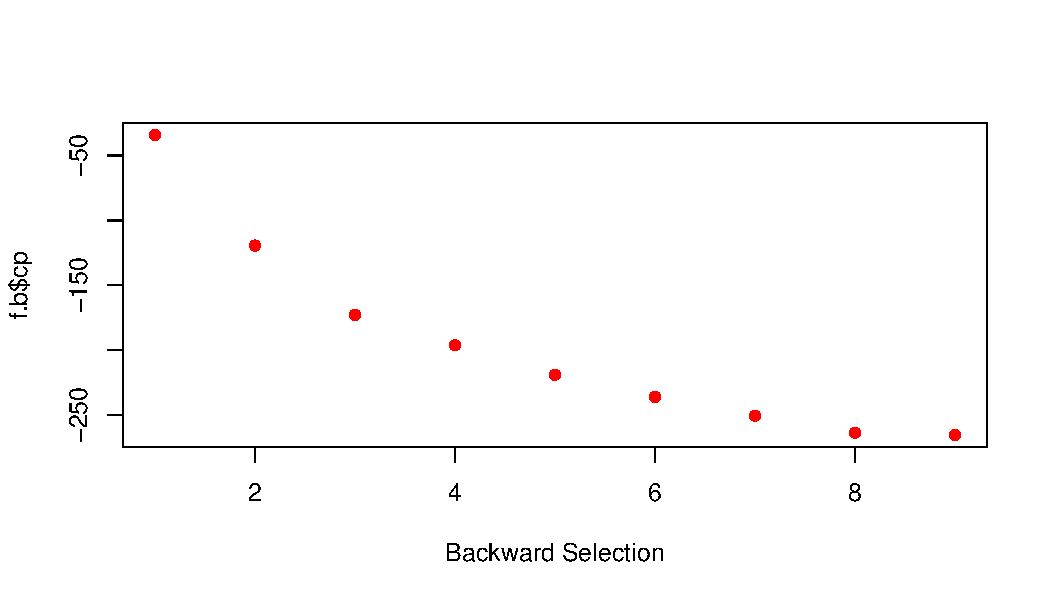
\includegraphics{hw3_fall2018_files/figure-latex/unnamed-chunk-17-1.pdf}

\begin{Shaded}
\begin{Highlighting}[]
\KeywordTok{plot}\NormalTok{(}\DecValTok{1}\OperatorTok{-}\NormalTok{fit1.roc}\OperatorTok{$}\NormalTok{specificities, fit1.roc}\OperatorTok{$}\NormalTok{sensitivities, }\DataTypeTok{col=}\StringTok{"red"}\NormalTok{, }\DataTypeTok{pch=}\DecValTok{16}\NormalTok{,}
     \DataTypeTok{xlab=}\StringTok{"False Positive"}\NormalTok{, }
     \DataTypeTok{ylab=}\StringTok{"Sensitivity"}\NormalTok{)}
\end{Highlighting}
\end{Shaded}

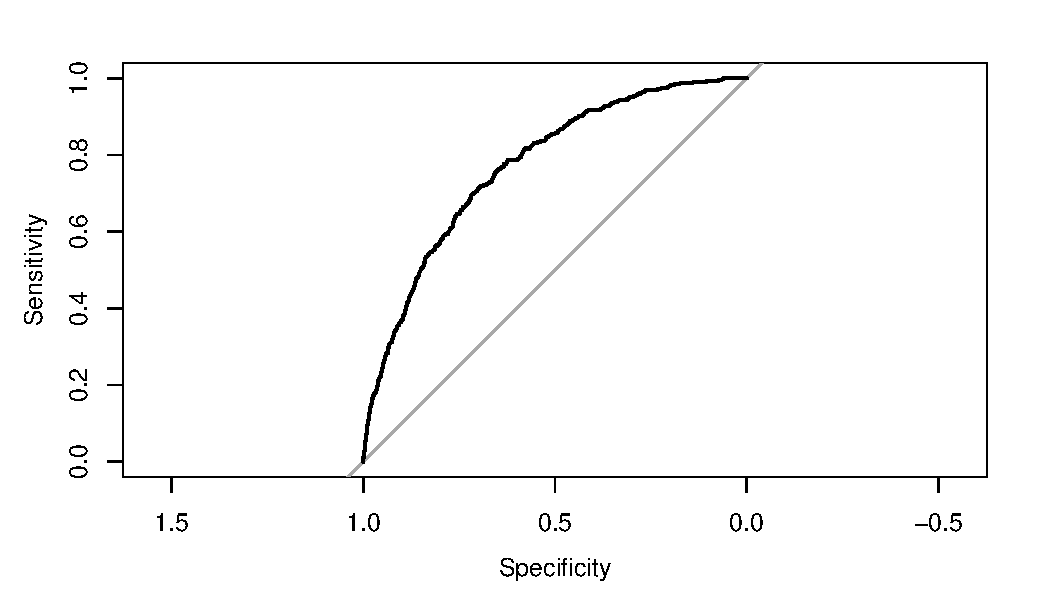
\includegraphics{hw3_fall2018_files/figure-latex/unnamed-chunk-17-2.pdf}

\section{Let us figure out the classifier such that False Positive Rate
is less than 0.1 and True Positive Rate is as high as
possible}\label{let-us-figure-out-the-classifier-such-that-false-positive-rate-is-less-than-0.1-and-true-positive-rate-is-as-high-as-possible}

\begin{Shaded}
\begin{Highlighting}[]
\CommentTok{#coords(fit1.roc, "best", ret = "threshold") This gives the best threshold value (will not be used here since we have constraints mentioned in the question)}
\NormalTok{coord_list <-}\StringTok{ }\KeywordTok{list}\NormalTok{()}
\NormalTok{coord_list[[}\DecValTok{1}\NormalTok{]] <-}\StringTok{ }\KeywordTok{coords}\NormalTok{(fit1.roc, }\DataTypeTok{x =} \StringTok{"all"}\NormalTok{)}
\NormalTok{coord_list[[}\DecValTok{1}\NormalTok{]]}
\end{Highlighting}
\end{Shaded}

\begin{verbatim}
##              all         all         all         all         all
## threshold   -Inf 0.101257641 0.107084595 0.110146435 0.113284712
## specificity    0 0.001841621 0.003683241 0.003683241 0.008287293
## sensitivity    1 1.000000000 1.000000000 0.996742671 0.996742671
##                     all        all        all        all        all
## threshold   0.116500696 0.11895694 0.12062431 0.12317078 0.12662733
## specificity 0.009208103 0.01104972 0.01381215 0.01565378 0.02578269
## sensitivity 0.996742671 0.99674267 0.99348534 0.99348534 0.98697068
##                   all        all        all        all        all
## threshold   0.1301665 0.13378939 0.13655419 0.13842945 0.14129099
## specificity 0.0534070 0.06169429 0.07366483 0.07826888 0.08747698
## sensitivity 0.9771987 0.97719870 0.96742671 0.96416938 0.96091205
##                   all       all       all       all       all       all
## threshold   0.1451718 0.1491408 0.1531988 0.1562928 0.1583894 0.1615856
## specificity 0.1049724 0.1574586 0.1740331 0.1988950 0.2145488 0.2421731
## sensitivity 0.9543974 0.9381107 0.9218241 0.8925081 0.8794788 0.8697068
##                   all       all       all       all       all       all
## threshold   0.1659162 0.1703392 0.1748555 0.1782954 0.1806239 0.1841700
## specificity 0.2615101 0.3305709 0.3499079 0.3756906 0.3922652 0.4217311
## sensitivity 0.8501629 0.8078176 0.7850163 0.7719870 0.7524430 0.7426710
##                   all       all       all       all       all       all
## threshold   0.1889694 0.1938642 0.1988546 0.2026514 0.2052186 0.2078099
## specificity 0.4511971 0.5248619 0.5469613 0.5718232 0.5874770 0.6049724
## sensitivity 0.7198697 0.6644951 0.6351792 0.6286645 0.6156352 0.5960912
##                   all       all       all       all       all       all
## threshold   0.2104252 0.2144023 0.2197773 0.2252484 0.2294057 0.2322131
## specificity 0.6058932 0.6243094 0.6740331 0.6878453 0.7090239 0.7228361
## sensitivity 0.5960912 0.5765472 0.5342020 0.5146580 0.5016287 0.4788274
##                   all       all       all       all       all       all
## threshold   0.2350444 0.2378996 0.2422357 0.2480881 0.2540345 0.2585468
## specificity 0.7412523 0.7421731 0.7541436 0.8038674 0.8103131 0.8167587
## sensitivity 0.4592834 0.4592834 0.4332248 0.3811075 0.3811075 0.3615635
##                   all       all       all       all       all       all
## threshold   0.2615898 0.2662060 0.2724292 0.2787427 0.2851452 0.2899965
## specificity 0.8305709 0.8342541 0.8443831 0.8692449 0.8793738 0.8885820
## sensitivity 0.3420195 0.3289902 0.3224756 0.2768730 0.2605863 0.2475570
##                   all       all       all       all       all       all
## threshold   0.2932632 0.2982114 0.3048720 0.3116153 0.3184394 0.3236021
## specificity 0.8968692 0.9023941 0.9060773 0.9217311 0.9272560 0.9346225
## sensitivity 0.2280130 0.2149837 0.2084691 0.1889251 0.1791531 0.1758958
##                   all       all       all       all       all       all
## threshold   0.3270730 0.3323220 0.3393760 0.3465020 0.3536976 0.3591322
## specificity 0.9392265 0.9410681 0.9429098 0.9530387 0.9539595 0.9558011
## sensitivity 0.1661238 0.1563518 0.1530945 0.1302932 0.1270358 0.1205212
##                   all       all       all        all        all        all
## threshold   0.3627798 0.3682866 0.3756744 0.38312062 0.39062204 0.39627780
## specificity 0.9576427 0.9585635 0.9594843 0.96685083 0.96685083 0.96777164
## sensitivity 0.1074919 0.1042345 0.1042345 0.09446254 0.09120521 0.08794788
##                    all        all       all        all        all
## threshold   0.40006716 0.40577782 0.4134256 0.42111526 0.42884344
## specificity 0.96961326 0.97053407 0.9723757 0.97790055 0.97790055
## sensitivity 0.08794788 0.08794788 0.0781759 0.07491857 0.07166124
##                    all        all        all        all        all
## threshold   0.43465963 0.43854940 0.44831790 0.46597603 0.47778528
## specificity 0.97882136 0.97974217 0.97974217 0.98618785 0.98802947
## sensitivity 0.06840391 0.06514658 0.05537459 0.04560261 0.04560261
##                    all        all        all        all        all
## threshold   0.48370720 0.49160854 0.50346653 0.51532192 0.52715437
## specificity 0.98802947 0.98802947 0.98987109 0.99079190 0.99263352
## sensitivity 0.04234528 0.03908795 0.02931596 0.02931596 0.02931596
##                    all        all        all         all         all
## threshold   0.54679130 0.56631246 0.59314953 0.630625886 0.659680208
## specificity 0.99263352 0.99447514 0.99539595 0.995395948 0.995395948
## sensitivity 0.01954397 0.01954397 0.01302932 0.006514658 0.003257329
##                   all       all       all       all       all all
## threshold   0.6772407 0.6942211 0.7107897 0.7236149 0.7390850 Inf
## specificity 0.9953959 0.9963168 0.9972376 0.9981584 0.9990792   1
## sensitivity 0.0000000 0.0000000 0.0000000 0.0000000 0.0000000   0
\end{verbatim}

\section{For False Positive Rate to be less than 0.1, Specificity has to
be more than 0.9. Based on the above table, we can see that for a
Specificity of 0.9, the classifier has a threhold of 0.298. Any
classifier chosen greater than this will increase specificity, but
decrease
sensitivity.}\label{for-false-positive-rate-to-be-less-than-0.1-specificity-has-to-be-more-than-0.9.-based-on-the-above-table-we-can-see-that-for-a-specificity-of-0.9-the-classifier-has-a-threhold-of-0.298.-any-classifier-chosen-greater-than-this-will-increase-specificity-but-decrease-sensitivity.}

\begin{enumerate}
\def\labelenumi{\alph{enumi}.}
\setcounter{enumi}{1}
\tightlist
\item
  Overlay two ROC curves: one from \texttt{fit1}, the other from
  \texttt{fit2}. Does one curve always contain the other curve? Is the
  AUC of one curve always larger than the AUC of the other one? Why or
  why not?
\end{enumerate}

\begin{Shaded}
\begin{Highlighting}[]
\NormalTok{fit2.roc<-}\StringTok{ }\KeywordTok{roc}\NormalTok{(hd_data.f}\OperatorTok{$}\NormalTok{HD, fit2}\OperatorTok{$}\NormalTok{fitted)}
\KeywordTok{plot}\NormalTok{(}\DecValTok{1}\OperatorTok{-}\NormalTok{fit1.roc}\OperatorTok{$}\NormalTok{specificities, fit1.roc}\OperatorTok{$}\NormalTok{sensitivities, }\DataTypeTok{col=}\StringTok{"red"}\NormalTok{, }\DataTypeTok{pch=}\DecValTok{16}\NormalTok{, }\DataTypeTok{cex=}\NormalTok{.}\DecValTok{7}\NormalTok{, }
     \DataTypeTok{xlab=}\StringTok{"False Positive"}\NormalTok{, }
     \DataTypeTok{ylab=}\StringTok{"Sensitivity"}\NormalTok{)}
\KeywordTok{points}\NormalTok{(}\DecValTok{1}\OperatorTok{-}\NormalTok{fit2.roc}\OperatorTok{$}\NormalTok{specificities, fit2.roc}\OperatorTok{$}\NormalTok{sensitivities, }\DataTypeTok{col=}\StringTok{"blue"}\NormalTok{, }\DataTypeTok{pch=}\DecValTok{16}\NormalTok{, }\DataTypeTok{cex=}\NormalTok{.}\DecValTok{6}\NormalTok{)}
\KeywordTok{title}\NormalTok{(}\StringTok{"Blue for fit2, Red for fit1"}\NormalTok{)}
\end{Highlighting}
\end{Shaded}

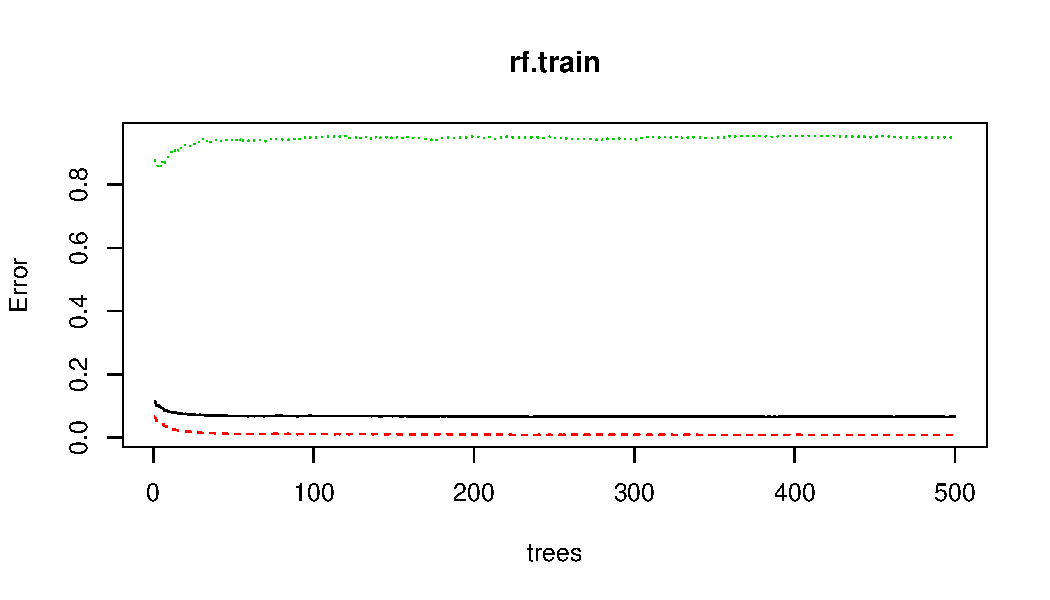
\includegraphics{hw3_fall2018_files/figure-latex/unnamed-chunk-19-1.pdf}

\subsection{fit2 curve (blue) contains the fit1 curve (red). Hence AUC
for fit2 curve is more than AUC for fit1. This is because for any
threshold value, fit2 offers a better predictive power than fit1 (as we
observed previously through AIC values and other tests). Thus, for any
given value of False Positive, fit2 always gives a higher True Positive
rate.}\label{fit2-curve-blue-contains-the-fit1-curve-red.-hence-auc-for-fit2-curve-is-more-than-auc-for-fit1.-this-is-because-for-any-threshold-value-fit2-offers-a-better-predictive-power-than-fit1-as-we-observed-previously-through-aic-values-and-other-tests.-thus-for-any-given-value-of-false-positive-fit2-always-gives-a-higher-true-positive-rate.}

\begin{enumerate}
\def\labelenumi{\alph{enumi}.}
\setcounter{enumi}{2}
\tightlist
\item
  Estimate the Positive Prediction Values and Negative Prediction Values
  for \texttt{fit1} and \texttt{fit2} using .5 as a threshold. Which
  model is more desirable if we prioritize the Positive Prediction
  values?
\end{enumerate}

\section{Preparing the Confusion Matrix for fit1 and
fit2:}\label{preparing-the-confusion-matrix-for-fit1-and-fit2}

\begin{Shaded}
\begin{Highlighting}[]
\NormalTok{fit1.pred <-}\StringTok{ }\KeywordTok{ifelse}\NormalTok{(fit1}\OperatorTok{$}\NormalTok{fitted }\OperatorTok{>}\StringTok{ }\DecValTok{1}\OperatorTok{/}\DecValTok{2}\NormalTok{, }\StringTok{"1"}\NormalTok{, }\StringTok{"0"}\NormalTok{)}
\NormalTok{fit2.pred <-}\StringTok{ }\KeywordTok{ifelse}\NormalTok{(fit2}\OperatorTok{$}\NormalTok{fitted }\OperatorTok{>}\StringTok{ }\DecValTok{1}\OperatorTok{/}\DecValTok{2}\NormalTok{, }\StringTok{"1"}\NormalTok{, }\StringTok{"0"}\NormalTok{)}
\NormalTok{fit1.confmat <-}\StringTok{ }\KeywordTok{table}\NormalTok{(fit1.pred, hd_data.f}\OperatorTok{$}\NormalTok{HD)}
\NormalTok{fit2.confmat <-}\StringTok{ }\KeywordTok{table}\NormalTok{(fit2.pred, hd_data.f}\OperatorTok{$}\NormalTok{HD)}
\NormalTok{fit1.confmat}
\end{Highlighting}
\end{Shaded}

\begin{verbatim}
##          
## fit1.pred    0    1
##         0 1075  298
##         1   11    9
\end{verbatim}

\begin{Shaded}
\begin{Highlighting}[]
\NormalTok{fit2.confmat}
\end{Highlighting}
\end{Shaded}

\begin{verbatim}
##          
## fit2.pred    0    1
##         0 1067  290
##         1   19   17
\end{verbatim}

\begin{Shaded}
\begin{Highlighting}[]
\NormalTok{fit1.pospre <-}\StringTok{ }\NormalTok{fit1.confmat[}\DecValTok{2}\NormalTok{,}\DecValTok{2}\NormalTok{]}\OperatorTok{/}\NormalTok{(fit1.confmat[}\DecValTok{2}\NormalTok{,}\DecValTok{1}\NormalTok{]}\OperatorTok{+}\NormalTok{fit1.confmat[}\DecValTok{2}\NormalTok{,}\DecValTok{2}\NormalTok{])}
\NormalTok{fit1.negpre <-}\StringTok{ }\NormalTok{fit1.confmat[}\DecValTok{1}\NormalTok{,}\DecValTok{1}\NormalTok{]}\OperatorTok{/}\NormalTok{(fit1.confmat[}\DecValTok{1}\NormalTok{,}\DecValTok{1}\NormalTok{]}\OperatorTok{+}\NormalTok{fit1.confmat[}\DecValTok{1}\NormalTok{,}\DecValTok{2}\NormalTok{])}
\NormalTok{fit2.pospre <-}\StringTok{ }\NormalTok{fit2.confmat[}\DecValTok{2}\NormalTok{,}\DecValTok{2}\NormalTok{]}\OperatorTok{/}\NormalTok{(fit2.confmat[}\DecValTok{2}\NormalTok{,}\DecValTok{1}\NormalTok{]}\OperatorTok{+}\NormalTok{fit2.confmat[}\DecValTok{2}\NormalTok{,}\DecValTok{2}\NormalTok{])}
\NormalTok{fit2.negpre <-}\StringTok{ }\NormalTok{fit2.confmat[}\DecValTok{1}\NormalTok{,}\DecValTok{1}\NormalTok{]}\OperatorTok{/}\NormalTok{(fit2.confmat[}\DecValTok{1}\NormalTok{,}\DecValTok{1}\NormalTok{]}\OperatorTok{+}\NormalTok{fit2.confmat[}\DecValTok{1}\NormalTok{,}\DecValTok{2}\NormalTok{])}
\NormalTok{fit1.pospre}
\end{Highlighting}
\end{Shaded}

\begin{verbatim}
## [1] 0.45
\end{verbatim}

\begin{Shaded}
\begin{Highlighting}[]
\NormalTok{fit1.negpre}
\end{Highlighting}
\end{Shaded}

\begin{verbatim}
## [1] 0.782957
\end{verbatim}

\begin{Shaded}
\begin{Highlighting}[]
\NormalTok{fit2.pospre}
\end{Highlighting}
\end{Shaded}

\begin{verbatim}
## [1] 0.4722222
\end{verbatim}

\begin{Shaded}
\begin{Highlighting}[]
\NormalTok{fit2.negpre}
\end{Highlighting}
\end{Shaded}

\begin{verbatim}
## [1] 0.7862933
\end{verbatim}

\section{As can be seen from above, fit2 is more desirable if we
prioritize positive prediction values since Positive Prediction rate for
fit2 is 0.47, which is superior than the Positive Prediction rate of
fit1, which is
0.45.}\label{as-can-be-seen-from-above-fit2-is-more-desirable-if-we-prioritize-positive-prediction-values-since-positive-prediction-rate-for-fit2-is-0.47-which-is-superior-than-the-positive-prediction-rate-of-fit1-which-is-0.45.}

\begin{enumerate}
\def\labelenumi{\alph{enumi}.}
\setcounter{enumi}{3}
\tightlist
\item
  (Optional/extra credit) For \texttt{fit1}: overlay two curves, but put
  the threshold over the probability function as the x-axis and positive
  prediction values and the negative prediction values as the y-axis.
  Overlay the same plot for \texttt{fit2}. Which model would you choose
  if the set of positive and negative prediction values are the
  concerns? If you can find an R package to do so, you may use it
  directly.
\end{enumerate}

\subsubsection{Part 3 - Bayes Rule}\label{part-3---bayes-rule}

Bayes rules with risk ratio \(\frac{a_{10}}{a_{01}}=10\) or
\(\frac{a_{10}}{a_{01}}=1\). Use your final model obtained from 1 B) to
build a class of linear classifiers.

\begin{enumerate}
\def\labelenumi{\alph{enumi}.}
\tightlist
\item
  Write down the linear boundary for the Bayes classifier if the risk
  ratio of \(a_{10}/a_{01}=10\).
\end{enumerate}

\begin{Shaded}
\begin{Highlighting}[]
\CommentTok{#Copying final model from 1B for reference}
\NormalTok{fit2 <-}\StringTok{ }\KeywordTok{glm}\NormalTok{(HD}\OperatorTok{~}\NormalTok{SBP }\OperatorTok{+}\StringTok{ }\NormalTok{SEX, hd_data.f, }\DataTypeTok{family=}\NormalTok{binomial)}
\KeywordTok{summary}\NormalTok{(fit2)}
\end{Highlighting}
\end{Shaded}

\begin{verbatim}
## 
## Call:
## glm(formula = HD ~ SBP + SEX, family = binomial, data = hd_data.f)
## 
## Deviance Residuals: 
##     Min       1Q   Median       3Q      Max  
## -1.6408  -0.7373  -0.5726  -0.4169   2.2452  
## 
## Coefficients:
##              Estimate Std. Error z value Pr(>|z|)    
## (Intercept) -4.570256   0.389727 -11.727  < 2e-16 ***
## SBP          0.018717   0.002324   8.053 8.07e-16 ***
## SEXMALE      0.903420   0.139762   6.464 1.02e-10 ***
## ---
## Signif. codes:  0 '***' 0.001 '**' 0.01 '*' 0.05 '.' 0.1 ' ' 1
## 
## (Dispersion parameter for binomial family taken to be 1)
## 
##     Null deviance: 1469.3  on 1392  degrees of freedom
## Residual deviance: 1373.8  on 1390  degrees of freedom
## AIC: 1379.8
## 
## Number of Fisher Scoring iterations: 4
\end{verbatim}

In this case, \(\frac{a_{0,1}}{a_{1,0}}=\frac{1}{10}=0.1\), therefore
\(prob(Y=1 \vert x) > \frac{0.1}{(1+0.1)}=0.09\) and
\(logit > \log(\frac{0.09}{0.91})=-2.31\)

For our fit model, \(-4.570+0.0187SBP+.9034Sex \geq -2.31\)

\(0.0187SBP+.9034Sex \geq -2.31+4.570\)

\$SBP \geq -48.31Sex + 120.855 \$ This is the linear boundary

\begin{Shaded}
\begin{Highlighting}[]
\CommentTok{#drawing the linear boundary}
\KeywordTok{plot}\NormalTok{(hd_data.f}\OperatorTok{$}\NormalTok{SEX, hd_data.f}\OperatorTok{$}\NormalTok{SBP, }\DataTypeTok{col=}\NormalTok{hd_data.f}\OperatorTok{$}\NormalTok{HD, }
     \DataTypeTok{pch=}\KeywordTok{as.numeric}\NormalTok{(hd_data.f}\OperatorTok{$}\NormalTok{HD)}\OperatorTok{+}\DecValTok{2}\NormalTok{,}
     \DataTypeTok{xlab=}\StringTok{"sex"}\NormalTok{, }\DataTypeTok{ylab=}\StringTok{"SBP"}\NormalTok{)}
\KeywordTok{legend}\NormalTok{(}\StringTok{"topleft"}\NormalTok{, }\DataTypeTok{legend=}\KeywordTok{c}\NormalTok{(}\StringTok{"HD=1"}\NormalTok{, }\StringTok{"HD=0"}\NormalTok{),}
       \DataTypeTok{lty=}\KeywordTok{c}\NormalTok{(}\DecValTok{1}\NormalTok{,}\DecValTok{1}\NormalTok{), }\DataTypeTok{lwd=}\KeywordTok{c}\NormalTok{(}\DecValTok{2}\NormalTok{,}\DecValTok{2}\NormalTok{), }\DataTypeTok{col=}\KeywordTok{c}\NormalTok{(}\StringTok{"red"}\NormalTok{, }\StringTok{"black"}\NormalTok{))}
\KeywordTok{abline}\NormalTok{(}\DataTypeTok{a=}\FloatTok{120.85}\NormalTok{, }\DataTypeTok{b=}\OperatorTok{-}\FloatTok{48.31}\NormalTok{, }\DataTypeTok{lwd=}\DecValTok{5}\NormalTok{, }\DataTypeTok{col=}\StringTok{"red"}\NormalTok{)}
\KeywordTok{title}\NormalTok{(}\StringTok{"Linear Boundary of the Bayes Rule, when a10/a01=10"}\NormalTok{)}
\end{Highlighting}
\end{Shaded}

\includegraphics{hw3_fall2018_files/figure-latex/unnamed-chunk-23-1.pdf}

\begin{enumerate}
\def\labelenumi{\alph{enumi}.}
\setcounter{enumi}{1}
\tightlist
\item
  What is your estimated weighted misclassification error for this given
  risk ratio?
\end{enumerate}

\begin{Shaded}
\begin{Highlighting}[]
\NormalTok{fit2.pred.bayes <-}\StringTok{ }\KeywordTok{rep}\NormalTok{(}\StringTok{"0"}\NormalTok{, }\DecValTok{1406}\NormalTok{)}
\NormalTok{fit2.pred.bayes[fit2}\OperatorTok{$}\NormalTok{fitted }\OperatorTok{>}\StringTok{ }\NormalTok{.}\DecValTok{09}\NormalTok{] =}\StringTok{ "1"}
\NormalTok{fit2.pred.bayes <-}\StringTok{ }\KeywordTok{as.factor}\NormalTok{(}\KeywordTok{ifelse}\NormalTok{(fit2}\OperatorTok{$}\NormalTok{fitted }\OperatorTok{>}\StringTok{ }\NormalTok{.}\DecValTok{09}\NormalTok{, }\StringTok{"1"}\NormalTok{, }\StringTok{"0"}\NormalTok{))}
\NormalTok{MCE.bayes=(}\KeywordTok{sum}\NormalTok{(}\DecValTok{5}\OperatorTok{*}\NormalTok{(fit2.pred.bayes[hd_data.f}\OperatorTok{$}\NormalTok{HD }\OperatorTok{==}\StringTok{ "1"}\NormalTok{] }\OperatorTok{!=}\StringTok{ "1"}\NormalTok{)) }
           \OperatorTok{+}\StringTok{ }\KeywordTok{sum}\NormalTok{(fit2.pred.bayes[hd_data.f}\OperatorTok{$}\NormalTok{HD }\OperatorTok{==}\StringTok{ "0"}\NormalTok{] }\OperatorTok{!=}\StringTok{ "0"}\NormalTok{))}\OperatorTok{/}\KeywordTok{length}\NormalTok{(hd_data.f}\OperatorTok{$}\NormalTok{HD)}
\NormalTok{MCE.bayes}
\end{Highlighting}
\end{Shaded}

\begin{verbatim}
## [1] 0.7343862
\end{verbatim}

\begin{enumerate}
\def\labelenumi{\alph{enumi}.}
\setcounter{enumi}{2}
\tightlist
\item
  Recall Liz, our patient from part 1. How would you classify her under
  this classifier?
\end{enumerate}

\section{First we need to calculate what will be the predicted value for
Liz under the fit2 model, then use the classifier to classify her
accordingly}\label{first-we-need-to-calculate-what-will-be-the-predicted-value-for-liz-under-the-fit2-model-then-use-the-classifier-to-classify-her-accordingly}

\begin{Shaded}
\begin{Highlighting}[]
\NormalTok{fit2.liz <-}\StringTok{ }\OperatorTok{-}\FloatTok{4.570256} \OperatorTok{+}\StringTok{ }\NormalTok{(}\FloatTok{0.018717}\OperatorTok{*}\DecValTok{110}\NormalTok{) }\OperatorTok{+}\StringTok{ }\NormalTok{(}\FloatTok{0.903420}\OperatorTok{*}\DecValTok{0}\NormalTok{)}
\NormalTok{fit2.liz <-}\StringTok{ }\KeywordTok{as.factor}\NormalTok{(}\KeywordTok{ifelse}\NormalTok{(fit2.liz }\OperatorTok{>}\StringTok{ }\NormalTok{.}\DecValTok{09}\NormalTok{, }\StringTok{"1"}\NormalTok{, }\StringTok{"0"}\NormalTok{))}
\NormalTok{  fit2.liz}
\end{Highlighting}
\end{Shaded}

\begin{verbatim}
## [1] 0
## Levels: 0
\end{verbatim}

\section{She would be classified as not at risk (level 0) under this
classifier}\label{she-would-be-classified-as-not-at-risk-level-0-under-this-classifier}

Now, draw two estimated curves where x = posterior threshold, and y =
misclassification errors, corresponding to the thresholding rule given
in x-axis.

\begin{enumerate}
\def\labelenumi{\alph{enumi}.}
\setcounter{enumi}{3}
\tightlist
\item
  Use weighted misclassification error, and set \(a_{10}/a_{01}=10\).
  How well does the Bayes rule classifier perform?
\end{enumerate}

\begin{Shaded}
\begin{Highlighting}[]
\NormalTok{i <-}\StringTok{ }\FloatTok{0.09}
\ControlFlowTok{while}\NormalTok{ (i }\OperatorTok{<}\NormalTok{.}\DecValTok{5}\NormalTok{) \{}
 
\NormalTok{fit2.pred.bayes <-}\StringTok{ }\KeywordTok{rep}\NormalTok{(}\StringTok{"0"}\NormalTok{, }\DecValTok{1406}\NormalTok{)}
\NormalTok{fit2.pred.bayes[fit2}\OperatorTok{$}\NormalTok{fitted }\OperatorTok{>}\StringTok{ }\NormalTok{i] =}\StringTok{ "1"}
\NormalTok{fit2.pred.bayes <-}\StringTok{ }\KeywordTok{as.factor}\NormalTok{(}\KeywordTok{ifelse}\NormalTok{(fit2}\OperatorTok{$}\NormalTok{fitted }\OperatorTok{>}\StringTok{ }\NormalTok{i, }\StringTok{"1"}\NormalTok{, }\StringTok{"0"}\NormalTok{))}
\NormalTok{MCE.bayes<-(}\KeywordTok{sum}\NormalTok{(}\DecValTok{5}\OperatorTok{*}\NormalTok{(fit2.pred.bayes[hd_data.f}\OperatorTok{$}\NormalTok{HD }\OperatorTok{==}\StringTok{ "1"}\NormalTok{] }\OperatorTok{!=}\StringTok{ "1"}\NormalTok{)) }
           \OperatorTok{+}\StringTok{ }\KeywordTok{sum}\NormalTok{(fit2.pred.bayes[hd_data.f}\OperatorTok{$}\NormalTok{HD }\OperatorTok{==}\StringTok{ "0"}\NormalTok{] }\OperatorTok{!=}\StringTok{ "0"}\NormalTok{))}\OperatorTok{/}\KeywordTok{length}\NormalTok{(hd_data.f}\OperatorTok{$}\NormalTok{HD)}
\NormalTok{MCE.i <-}\StringTok{ }\NormalTok{i}
\NormalTok{i <-}\StringTok{ }\NormalTok{i}\OperatorTok{+}\FloatTok{0.01}
\NormalTok{\}}

\KeywordTok{plot}\NormalTok{(MCE.bayes }\OperatorTok{~}\StringTok{ }\NormalTok{MCE.i,}\DataTypeTok{xlab=}\StringTok{"threshold"}\NormalTok{, }\DataTypeTok{ylab=}\StringTok{"MCE"}\NormalTok{ )}
\end{Highlighting}
\end{Shaded}

\includegraphics{hw3_fall2018_files/figure-latex/unnamed-chunk-26-1.pdf}

\begin{enumerate}
\def\labelenumi{\alph{enumi}.}
\setcounter{enumi}{4}
\tightlist
\item
  Use weighted misclassification error, and set \(a_{10}/a_{01}=1\). How
  well does the Bayes rule classifier perform?
\end{enumerate}

\begin{Shaded}
\begin{Highlighting}[]
\NormalTok{fit2.pred.bayes <-}\StringTok{ }\KeywordTok{rep}\NormalTok{(}\StringTok{"0"}\NormalTok{, }\DecValTok{1406}\NormalTok{)}
\NormalTok{fit2.pred.bayes[fit2}\OperatorTok{$}\NormalTok{fitted }\OperatorTok{>}\StringTok{ }\NormalTok{.}\DecValTok{5}\NormalTok{] =}\StringTok{ "1"}
\NormalTok{fit2.pred.bayes <-}\StringTok{ }\KeywordTok{as.factor}\NormalTok{(}\KeywordTok{ifelse}\NormalTok{(fit2}\OperatorTok{$}\NormalTok{fitted }\OperatorTok{>}\StringTok{ }\NormalTok{.}\DecValTok{5}\NormalTok{, }\StringTok{"1"}\NormalTok{, }\StringTok{"0"}\NormalTok{))}
\NormalTok{MCE.bayes<-(}\KeywordTok{sum}\NormalTok{(}\DecValTok{5}\OperatorTok{*}\NormalTok{(fit2.pred.bayes[hd_data.f}\OperatorTok{$}\NormalTok{HD }\OperatorTok{==}\StringTok{ "1"}\NormalTok{] }\OperatorTok{!=}\StringTok{ "1"}\NormalTok{)) }
           \OperatorTok{+}\StringTok{ }\KeywordTok{sum}\NormalTok{(fit2.pred.bayes[hd_data.f}\OperatorTok{$}\NormalTok{HD }\OperatorTok{==}\StringTok{ "0"}\NormalTok{] }\OperatorTok{!=}\StringTok{ "0"}\NormalTok{))}\OperatorTok{/}\KeywordTok{length}\NormalTok{(hd_data.f}\OperatorTok{$}\NormalTok{HD)}

\KeywordTok{plot}\NormalTok{(}\FloatTok{0.5}\NormalTok{,MCE.bayes,}\DataTypeTok{xlab=}\StringTok{"threshold"}\NormalTok{, }\DataTypeTok{ylab=}\StringTok{"MCE"}\NormalTok{ )}
\end{Highlighting}
\end{Shaded}

\includegraphics{hw3_fall2018_files/figure-latex/unnamed-chunk-27-1.pdf}

\subsection{Problem 2}\label{problem-2}

How well can we predict whether a bill will be passed by the
legislature?

Hundreds to thousands of bills are written each year in Pennsylvania.
Some are long, others are short. Most of the bills do not even get to be
voted on (``sent to the floor''). The chamber meets for 2-year sessions.
Bills that are not voted on before the end of the session (or which are
voted on but lose the vote) are declared dead. Most bills die. In this
study we examine about 8000 bills proposed since 2009, with the goal of
building a classifier which has decent power to forecast which bills are
likely to be passed.

We have available some information about 8011 bills pertaining to
legislation introduced into the Pennsylvania House of Representatives.
The goal is to predict which proposals will pass the House. Here is some
information about the data:

The response is the variable called \texttt{status.}
\texttt{Bill:passed} means that the bill passed the House;
\texttt{governor:signed} means that the bill passed both chambers
(including the House) and was enacted into law;
\texttt{governor:received} means that the bill has passed both chambers
and was placed before the governor for consideration. All three of these
statuses signify a success or a PASS (Meaning that the legislature
passed the bill. This does not require it becoming law). All other
outcomes are failures.

Here are the rest of the columns:

\begin{itemize}
\tightlist
\item
  \texttt{Session} : in which legislative session was the bill
  introduced
\item
  \texttt{Sponsor\_party} : the party of the legislator who sponsored
  the bill (every bill has a sponsor)
\item
  \texttt{Bill\_id} : of the form HB-{[}bill number{]}-{[}session{]},
  e.g., \texttt{HB-2661-2013-2014} for the 2661st House Bill introduced
  in the 2013-2014 session.
\item
  \texttt{Num\_cosponsors} : how many legislators cosponsored the bill
\item
  \texttt{Num\_d\_cosponsors} : how many Democrats cosponsored the bill
\item
  \texttt{Num\_r\_cosponsors} : how many Republicans cosponsored the
  bill
\item
  \texttt{Title\_word\_count} : how many words are in the bill's title
\item
  \texttt{Originating\_committee} : most bills are sent (``referred'')
  to a committee of jurisdiction (like the transportation committee,
  banking \& insurance committee, agriculture \& rural affairs
  committee) where they are discussed and amended. The originating
  committee is the committee to which a bill is referred.
\item
  \texttt{Day\_of\_week\_introduced} : on what day the bill was
  introduced in the House (1 is Monday)
\item
  \texttt{Num\_amendments} : how many amendments the bill has
\item
  \texttt{Is\_sponsor\_in\_leadership} : does the sponsor of the bill
  hold a position inside the House (such as speaker, majority leader,
  etc.)
\item
  \texttt{num\_originating\_committee\_cosponsors} : how many cosponsors
  sit on the committee to which the bill is referred
\item
  \texttt{num\_originating\_committee\_cosponsors\_r} : how many
  Republican cosponsors sit on the committee to which the bill is
  referred
\item
  \texttt{num\_originating\_committee\_cosponsors\_d} - how many
  Democratic cosponsors sit on the committee to which the bill is
  referred
\end{itemize}

The data you can use to build the classifier is called
\texttt{Bills.subset}. It contains 7011 records from the full data set.
I took a random sample of 1000 bills from the 2013-2014 session as
testing data set in order to test the quality of your classifier, it is
called \texttt{Bills.subset.test.}

Your job is to choose a best set of classifiers such that

\begin{itemize}
\tightlist
\item
  The testing ROC curve pushes to the upper left corner the most, and
  has a competitive AUC value.
\item
  Propose a reasonable loss function, and report the Bayes rule together
  with its weighted MIC.
\item
  You may also create some sensible variables based on the predictors or
  make other transformations to improve the performance of your
  classifier.
\end{itemize}

Here is what you need to report:

\begin{enumerate}
\def\labelenumi{\arabic{enumi}.}
\tightlist
\item
  Write a summary about the goal of the project. Give some background
  information. If desired, you may go online to find out more
  information.
\end{enumerate}

The objective of this project is to create a model which can predict a
legislative bill's likelihood of passing. This information would be
valuable to have (a) at the time the bill is introduced, to see how
optomistic we should be about its success, or (b) before the bill is
even introduced, to try to create a more effective environment within
which the bill could be introduced. For example, if our model indicates
that introducing a bill on a Tuesday is more likely to lead to success
than introducing the bill on a Monday, then the necessary preparations
can be made for a Tuesday introduction.

The model's implications could even be valuable for bills already under
consideration. For example, if bipartisan support for a bill makes it
much more likely to pass, then the bill sponsors could look for ways to
attract support from the opposing party.

This project should be of interest not just to legislators, but to
involved citizens across the country. Applying analytics to the
legislative process will yield interesting insights which could give one
party or cause a leg up if they are able to apply the model implications
to real-world issues (e.g.~via lobbying).

\begin{enumerate}
\def\labelenumi{\arabic{enumi}.}
\setcounter{enumi}{1}
\tightlist
\item
  Give a preliminary summary of the data.
\end{enumerate}

\begin{Shaded}
\begin{Highlighting}[]
\CommentTok{# Read in the data}
\NormalTok{bills_train <-}\StringTok{ }\KeywordTok{read.csv}\NormalTok{(}\StringTok{"Bills.subset.csv"}\NormalTok{)}

\CommentTok{# View variable names}
\KeywordTok{names}\NormalTok{(bills_train)}
\end{Highlighting}
\end{Shaded}

\begin{verbatim}
##  [1] "bill_id"                               
##  [2] "sponsor_party"                         
##  [3] "session"                               
##  [4] "num_cosponsors"                        
##  [5] "num_d_cosponsors"                      
##  [6] "num_r_cosponsors"                      
##  [7] "title_word_count"                      
##  [8] "originating_committee"                 
##  [9] "day.of.week.introduced"                
## [10] "num_amendments"                        
## [11] "status"                                
## [12] "is_sponsor_in_leadership"              
## [13] "num_originating_committee_cosponsors"  
## [14] "num_originating_committee_cosponsors_r"
## [15] "num_originating_committee_cosponsors_d"
\end{verbatim}

\begin{Shaded}
\begin{Highlighting}[]
\CommentTok{# Simple overview of variable components}
\KeywordTok{str}\NormalTok{(bills_train)}
\end{Highlighting}
\end{Shaded}

\begin{verbatim}
## 'data.frame':    7011 obs. of  15 variables:
##  $ bill_id                               : Factor w/ 7011 levels "HB-1-2009-2010",..: 5591 3720 4699 3055 130 2342 548 245 5013 6709 ...
##  $ sponsor_party                         : Factor w/ 3 levels "","Democratic",..: 3 2 2 2 2 2 3 2 3 3 ...
##  $ session                               : Factor w/ 4 levels "2009-2010","2009-2010 Special Session #1 (Transportation)",..: 1 1 1 1 1 1 1 1 1 1 ...
##  $ num_cosponsors                        : int  32 0 9 30 4 0 34 4 9 61 ...
##  $ num_d_cosponsors                      : int  0 0 6 24 4 0 14 3 2 22 ...
##  $ num_r_cosponsors                      : int  32 0 3 6 0 0 20 1 7 39 ...
##  $ title_word_count                      : int  27 50 20 25 29 30 32 25 20 46 ...
##  $ originating_committee                 : Factor w/ 26 levels "","PAC000001",..: 1 6 3 11 3 8 1 3 1 1 ...
##  $ day.of.week.introduced                : int  3 5 1 1 1 3 5 2 1 4 ...
##  $ num_amendments                        : int  0 0 0 1 0 0 2 0 0 1 ...
##  $ status                                : Factor w/ 10 levels "","amendment:passed",..: 8 10 8 8 8 8 8 8 8 2 ...
##  $ is_sponsor_in_leadership              : int  0 0 0 0 0 0 0 0 0 0 ...
##  $ num_originating_committee_cosponsors  : int  0 0 3 3 0 0 0 0 0 0 ...
##  $ num_originating_committee_cosponsors_r: int  0 0 1 1 0 0 0 0 0 0 ...
##  $ num_originating_committee_cosponsors_d: int  0 0 2 2 0 0 0 0 0 0 ...
\end{verbatim}

\begin{Shaded}
\begin{Highlighting}[]
\CommentTok{# Summary of variables}
\KeywordTok{summary}\NormalTok{(bills_train)}
\end{Highlighting}
\end{Shaded}

\begin{verbatim}
##                                                 bill_id    
##  HB-1-2009-2010                                     :   1  
##  HB-1-2009-2010 Special Session #1 (Transportation) :   1  
##  HB-1-2011-2012                                     :   1  
##  HB-10-2009-2010                                    :   1  
##  HB-10-2009-2010 Special Session #1 (Transportation):   1  
##  HB-10-2011-2012                                    :   1  
##  (Other)                                            :7005  
##     sponsor_party                                           session    
##            : 102   2009-2010                                    :2787  
##  Democratic:3213   2009-2010 Special Session #1 (Transportation):  23  
##  Republican:3696   2011-2012                                    :2709  
##                    2013-2014                                    :1492  
##                                                                        
##                                                                        
##                                                                        
##  num_cosponsors  num_d_cosponsors num_r_cosponsors title_word_count
##  Min.   :  0.0   Min.   : 0.00    Min.   : 0.00    Min.   :  6.00  
##  1st Qu.: 11.0   1st Qu.: 3.00    1st Qu.: 3.00    1st Qu.: 22.00  
##  Median : 20.0   Median : 8.00    Median : 8.00    Median : 27.00  
##  Mean   : 23.5   Mean   :10.43    Mean   :13.08    Mean   : 33.95  
##  3rd Qu.: 32.0   3rd Qu.:15.00    3rd Qu.:19.00    3rd Qu.: 34.00  
##  Max.   :165.0   Max.   :90.00    Max.   :99.00    Max.   :751.00  
##                                                                    
##  originating_committee day.of.week.introduced num_amendments  
##  PAC000004:1047        Min.   :1.000          Min.   :0.0000  
##  PAC000012: 810        1st Qu.:2.000          1st Qu.:0.0000  
##  PAC000001: 677        Median :3.000          Median :0.0000  
##  PAC000016: 622        Mean   :2.724          Mean   :0.1774  
##  PAC000017: 526        3rd Qu.:4.000          3rd Qu.:0.0000  
##  PAC000007: 329        Max.   :6.000          Max.   :8.0000  
##  (Other)  :3000        NA's   :5                              
##                 status     is_sponsor_in_leadership
##  committee:referred:6113   Min.   :0.0000          
##  governor:signed   : 428   1st Qu.:0.0000          
##  bill:reading:1    : 234   Median :1.0000          
##  committee:passed  : 106   Mean   :0.5904          
##  bill:reading:2    :  73   3rd Qu.:1.0000          
##  bill:passed       :  31   Max.   :1.0000          
##  (Other)           :  26                           
##  num_originating_committee_cosponsors
##  Min.   : 0.00                       
##  1st Qu.: 0.00                       
##  Median : 1.00                       
##  Mean   : 2.05                       
##  3rd Qu.: 3.00                       
##  Max.   :19.00                       
##                                      
##  num_originating_committee_cosponsors_r
##  Min.   : 0.000                        
##  1st Qu.: 0.000                        
##  Median : 1.000                        
##  Mean   : 1.342                        
##  3rd Qu.: 2.000                        
##  Max.   :14.000                        
##                                        
##  num_originating_committee_cosponsors_d
##  Min.   :0.0000                        
##  1st Qu.:0.0000                        
##  Median :0.0000                        
##  Mean   :0.7082                        
##  3rd Qu.:1.0000                        
##  Max.   :8.0000                        
## 
\end{verbatim}

\begin{Shaded}
\begin{Highlighting}[]
\CommentTok{# Create the target variable -- pass or fail}
\NormalTok{bills_train}\OperatorTok{$}\NormalTok{pass <-}\StringTok{ }\DecValTok{0}
\NormalTok{bills_train}\OperatorTok{$}\NormalTok{pass[bills_train}\OperatorTok{$}\NormalTok{status }\OperatorTok{==}\StringTok{ 'bill:passed'}\NormalTok{] <-}\StringTok{ }\DecValTok{1}
\NormalTok{bills_train}\OperatorTok{$}\NormalTok{pass[bills_train}\OperatorTok{$}\NormalTok{status }\OperatorTok{==}\StringTok{ 'governor:signed'}\NormalTok{] <-}\StringTok{ }\DecValTok{1}
\NormalTok{bills_train}\OperatorTok{$}\NormalTok{pass[bills_train}\OperatorTok{$}\NormalTok{status }\OperatorTok{==}\StringTok{ 'governor:received'}\NormalTok{] <-}\StringTok{ }\DecValTok{1}
\KeywordTok{summary}\NormalTok{(bills_train}\OperatorTok{$}\NormalTok{pass)}
\end{Highlighting}
\end{Shaded}

\begin{verbatim}
##    Min. 1st Qu.  Median    Mean 3rd Qu.    Max. 
## 0.00000 0.00000 0.00000 0.06604 0.00000 1.00000
\end{verbatim}

By looking at the mean of the target ``pass'' variable that we have
created, we see that only 6.6\% of the bills which are introduced end up
passing.

\begin{enumerate}
\def\labelenumi{\arabic{enumi}.}
\setcounter{enumi}{2}
\tightlist
\item
  Based on the data available to you, you need to build a classifier.
  Provide the following information:

  \begin{itemize}
  \tightlist
  \item
    The process of building your classifier
  \item
    Methods explored, and why you chose your final model
  \item
    Did you use a training and test set to build your classifier using
    the training data? If so, describe the process including information
    about the size of your training and test sets.
  \item
    What is the criterion being used to build your classifier?
  \item
    How do you estimate the quality of your classifier?
  \end{itemize}
\end{enumerate}

\begin{Shaded}
\begin{Highlighting}[]
\CommentTok{# fit cosponsor variables}
\NormalTok{fit1 <-}\StringTok{ }\KeywordTok{glm}\NormalTok{(pass }\OperatorTok{~}\StringTok{ }\NormalTok{num_cosponsors }\OperatorTok{+}\StringTok{ }\NormalTok{num_d_cosponsors }\OperatorTok{+}\StringTok{ }\NormalTok{num_r_cosponsors }\OperatorTok{+}\StringTok{ }\NormalTok{num_originating_committee_cosponsors }\OperatorTok{+}\StringTok{ }\NormalTok{num_originating_committee_cosponsors_r }\OperatorTok{+}\StringTok{ }\NormalTok{num_originating_committee_cosponsors_d, }\DataTypeTok{data=}\NormalTok{bills_train, }\DataTypeTok{family=}\KeywordTok{binomial}\NormalTok{())}
\KeywordTok{summary}\NormalTok{(fit1) }\CommentTok{# show results}
\end{Highlighting}
\end{Shaded}

\begin{verbatim}
## 
## Call:
## glm(formula = pass ~ num_cosponsors + num_d_cosponsors + num_r_cosponsors + 
##     num_originating_committee_cosponsors + num_originating_committee_cosponsors_r + 
##     num_originating_committee_cosponsors_d, family = binomial(), 
##     data = bills_train)
## 
## Deviance Residuals: 
##     Min       1Q   Median       3Q      Max  
## -1.0246  -0.3809  -0.3343  -0.3070   2.7151  
## 
## Coefficients: (2 not defined because of singularities)
##                                         Estimate Std. Error z value
## (Intercept)                            -3.031245   0.082399 -36.787
## num_cosponsors                          0.011941   0.004484   2.663
## num_d_cosponsors                       -0.023225   0.008222  -2.825
## num_r_cosponsors                              NA         NA      NA
## num_originating_committee_cosponsors    0.167777   0.050472   3.324
## num_originating_committee_cosponsors_r -0.054925   0.065438  -0.839
## num_originating_committee_cosponsors_d        NA         NA      NA
##                                        Pr(>|z|)    
## (Intercept)                             < 2e-16 ***
## num_cosponsors                         0.007738 ** 
## num_d_cosponsors                       0.004730 ** 
## num_r_cosponsors                             NA    
## num_originating_committee_cosponsors   0.000887 ***
## num_originating_committee_cosponsors_r 0.401281    
## num_originating_committee_cosponsors_d       NA    
## ---
## Signif. codes:  0 '***' 0.001 '**' 0.01 '*' 0.05 '.' 0.1 ' ' 1
## 
## (Dispersion parameter for binomial family taken to be 1)
## 
##     Null deviance: 3411.1  on 7010  degrees of freedom
## Residual deviance: 3322.5  on 7006  degrees of freedom
## AIC: 3332.5
## 
## Number of Fisher Scoring iterations: 5
\end{verbatim}

\begin{Shaded}
\begin{Highlighting}[]
\CommentTok{# fit non-cosponsor variables}
\NormalTok{fit2 <-}\StringTok{ }\KeywordTok{glm}\NormalTok{(pass }\OperatorTok{~}\StringTok{ }\NormalTok{sponsor_party }\OperatorTok{+}\StringTok{ }\NormalTok{session }\OperatorTok{+}\StringTok{ }\NormalTok{title_word_count }\OperatorTok{+}\StringTok{ }\NormalTok{originating_committee }\OperatorTok{+}\StringTok{ }\NormalTok{day.of.week.introduced }\OperatorTok{+}\StringTok{ }\NormalTok{num_amendments }\OperatorTok{+}\StringTok{ }\NormalTok{is_sponsor_in_leadership, }\DataTypeTok{data=}\NormalTok{bills_train, }\DataTypeTok{family=}\KeywordTok{binomial}\NormalTok{())}
\KeywordTok{summary}\NormalTok{(fit2) }\CommentTok{# show results}
\end{Highlighting}
\end{Shaded}

\begin{verbatim}
## 
## Call:
## glm(formula = pass ~ sponsor_party + session + title_word_count + 
##     originating_committee + day.of.week.introduced + num_amendments + 
##     is_sponsor_in_leadership, family = binomial(), data = bills_train)
## 
## Deviance Residuals: 
##     Min       1Q   Median       3Q      Max  
## -3.1040  -0.2773  -0.1813  -0.1219   3.1777  
## 
## Coefficients:
##                                                        Estimate Std. Error
## (Intercept)                                           -6.553496   1.170822
## sponsor_partyDemocratic                                1.141101   1.070369
## sponsor_partyRepublican                                1.955559   1.066506
## session2009-2010 Special Session #1 (Transportation) -11.349491 298.079519
## session2011-2012                                       1.035794   0.424721
## session2013-2014                                       1.038678   0.434490
## title_word_count                                       0.004720   0.001169
## originating_committeePAC000001                         1.887603   0.493695
## originating_committeePAC000004                         0.607766   0.501670
## originating_committeePAC000005                         1.245614   0.554099
## originating_committeePAC000007                         1.536742   0.513295
## originating_committeePAC000008                         2.993151   0.508659
## originating_committeePAC000010                         0.029338   0.622444
## originating_committeePAC000012                         0.115505   0.532820
## originating_committeePAC000015                         1.660406   0.590676
## originating_committeePAC000016                        -0.550298   0.607834
## originating_committeePAC000017                        -0.574121   0.617079
## originating_committeePAC000019                         1.117554   0.598886
## originating_committeePAC000035                         0.788729   0.659192
## originating_committeePAC000040                        -1.397454   0.851893
## originating_committeePAC000099                         0.827584   0.660587
## originating_committeePAC000129                         1.124096   0.547253
## originating_committeePAC000141                         0.090606   0.634912
## originating_committeePAC000165                       -11.179088 414.857019
## originating_committeePAC000190                         1.306243   0.607048
## originating_committeePAC000215                         2.135535   0.685683
## originating_committeePAC000229                         1.733595   0.550091
## originating_committeePAC000244                        -0.842565   0.876238
## originating_committeePAC000246                         0.889633   0.622370
## originating_committeePAC000263                         0.415435   0.649253
## originating_committeePAC000264                         0.353089   0.595957
## originating_committeePAC000265                        -0.665699   1.107935
## day.of.week.introduced                                 0.014022   0.044391
## num_amendments                                         1.845034   0.083089
## is_sponsor_in_leadership                              -0.519720   0.411673
##                                                      z value Pr(>|z|)    
## (Intercept)                                           -5.597 2.18e-08 ***
## sponsor_partyDemocratic                                1.066 0.286386    
## sponsor_partyRepublican                                1.834 0.066711 .  
## session2009-2010 Special Session #1 (Transportation)  -0.038 0.969628    
## session2011-2012                                       2.439 0.014738 *  
## session2013-2014                                       2.391 0.016822 *  
## title_word_count                                       4.037 5.40e-05 ***
## originating_committeePAC000001                         3.823 0.000132 ***
## originating_committeePAC000004                         1.211 0.225710    
## originating_committeePAC000005                         2.248 0.024576 *  
## originating_committeePAC000007                         2.994 0.002755 ** 
## originating_committeePAC000008                         5.884 4.00e-09 ***
## originating_committeePAC000010                         0.047 0.962407    
## originating_committeePAC000012                         0.217 0.828379    
## originating_committeePAC000015                         2.811 0.004938 ** 
## originating_committeePAC000016                        -0.905 0.365284    
## originating_committeePAC000017                        -0.930 0.352171    
## originating_committeePAC000019                         1.866 0.062034 .  
## originating_committeePAC000035                         1.197 0.231498    
## originating_committeePAC000040                        -1.640 0.100920    
## originating_committeePAC000099                         1.253 0.210278    
## originating_committeePAC000129                         2.054 0.039969 *  
## originating_committeePAC000141                         0.143 0.886523    
## originating_committeePAC000165                        -0.027 0.978502    
## originating_committeePAC000190                         2.152 0.031413 *  
## originating_committeePAC000215                         3.114 0.001843 ** 
## originating_committeePAC000229                         3.151 0.001625 ** 
## originating_committeePAC000244                        -0.962 0.336265    
## originating_committeePAC000246                         1.429 0.152881    
## originating_committeePAC000263                         0.640 0.522260    
## originating_committeePAC000264                         0.592 0.553533    
## originating_committeePAC000265                        -0.601 0.547942    
## day.of.week.introduced                                 0.316 0.752096    
## num_amendments                                        22.206  < 2e-16 ***
## is_sponsor_in_leadership                              -1.262 0.206783    
## ---
## Signif. codes:  0 '***' 0.001 '**' 0.01 '*' 0.05 '.' 0.1 ' ' 1
## 
## (Dispersion parameter for binomial family taken to be 1)
## 
##     Null deviance: 3410.5  on 7005  degrees of freedom
## Residual deviance: 2227.9  on 6971  degrees of freedom
##   (5 observations deleted due to missingness)
## AIC: 2297.9
## 
## Number of Fisher Scoring iterations: 14
\end{verbatim}

\begin{Shaded}
\begin{Highlighting}[]
\CommentTok{# fit all variables}
\NormalTok{fit3 <-}\StringTok{ }\KeywordTok{glm}\NormalTok{(pass }\OperatorTok{~}\StringTok{ }\NormalTok{sponsor_party }\OperatorTok{+}\StringTok{ }\NormalTok{session }\OperatorTok{+}\StringTok{ }\NormalTok{num_cosponsors }\OperatorTok{+}\StringTok{ }\NormalTok{num_d_cosponsors }\OperatorTok{+}\StringTok{ }\NormalTok{num_r_cosponsors }\OperatorTok{+}\StringTok{ }\NormalTok{title_word_count }\OperatorTok{+}\StringTok{ }\NormalTok{originating_committee }\OperatorTok{+}\StringTok{ }\NormalTok{day.of.week.introduced }\OperatorTok{+}\StringTok{ }\NormalTok{num_amendments }\OperatorTok{+}\StringTok{ }\NormalTok{is_sponsor_in_leadership }\OperatorTok{+}\StringTok{ }\NormalTok{num_originating_committee_cosponsors }\OperatorTok{+}\StringTok{ }\NormalTok{num_originating_committee_cosponsors_r }\OperatorTok{+}\StringTok{ }\NormalTok{num_originating_committee_cosponsors_d, }\DataTypeTok{data=}\NormalTok{bills_train, }\DataTypeTok{family=}\KeywordTok{binomial}\NormalTok{())}
\KeywordTok{summary}\NormalTok{(fit3) }\CommentTok{# show results}
\end{Highlighting}
\end{Shaded}

\begin{verbatim}
## 
## Call:
## glm(formula = pass ~ sponsor_party + session + num_cosponsors + 
##     num_d_cosponsors + num_r_cosponsors + title_word_count + 
##     originating_committee + day.of.week.introduced + num_amendments + 
##     is_sponsor_in_leadership + num_originating_committee_cosponsors + 
##     num_originating_committee_cosponsors_r + num_originating_committee_cosponsors_d, 
##     family = binomial(), data = bills_train)
## 
## Deviance Residuals: 
##     Min       1Q   Median       3Q      Max  
## -3.1085  -0.2793  -0.1854  -0.1237   3.2259  
## 
## Coefficients: (2 not defined because of singularities)
##                                                        Estimate Std. Error
## (Intercept)                                          -6.737e+00  1.184e+00
## sponsor_partyDemocratic                               1.098e+00  1.075e+00
## sponsor_partyRepublican                               1.968e+00  1.067e+00
## session2009-2010 Special Session #1 (Transportation) -1.121e+01  2.975e+02
## session2011-2012                                      9.717e-01  4.273e-01
## session2013-2014                                      9.738e-01  4.388e-01
## num_cosponsors                                       -9.591e-04  6.500e-03
## num_d_cosponsors                                      1.208e-02  1.189e-02
## num_r_cosponsors                                             NA         NA
## title_word_count                                      4.787e-03  1.172e-03
## originating_committeePAC000001                        1.903e+00  5.089e-01
## originating_committeePAC000004                        6.235e-01  5.255e-01
## originating_committeePAC000005                        1.133e+00  5.787e-01
## originating_committeePAC000007                        1.633e+00  5.286e-01
## originating_committeePAC000008                        3.089e+00  5.395e-01
## originating_committeePAC000010                        4.311e-02  6.345e-01
## originating_committeePAC000012                        1.799e-01  5.493e-01
## originating_committeePAC000015                        1.632e+00  6.198e-01
## originating_committeePAC000016                       -5.563e-01  6.270e-01
## originating_committeePAC000017                       -5.834e-01  6.319e-01
## originating_committeePAC000019                        1.107e+00  6.328e-01
## originating_committeePAC000035                        7.666e-01  6.650e-01
## originating_committeePAC000040                       -1.299e+00  8.596e-01
## originating_committeePAC000099                        8.623e-01  6.795e-01
## originating_committeePAC000129                        1.091e+00  5.822e-01
## originating_committeePAC000141                        1.083e-01  6.470e-01
## originating_committeePAC000165                       -1.107e+01  4.147e+02
## originating_committeePAC000190                        1.366e+00  6.216e-01
## originating_committeePAC000215                        2.108e+00  7.121e-01
## originating_committeePAC000229                        1.698e+00  5.851e-01
## originating_committeePAC000244                       -8.255e-01  8.938e-01
## originating_committeePAC000246                        9.554e-01  6.319e-01
## originating_committeePAC000263                        3.793e-01  6.664e-01
## originating_committeePAC000264                        3.554e-01  6.210e-01
## originating_committeePAC000265                       -7.953e-01  1.114e+00
## day.of.week.introduced                                1.505e-02  4.451e-02
## num_amendments                                        1.808e+00  8.427e-02
## is_sponsor_in_leadership                             -4.544e-01  4.137e-01
## num_originating_committee_cosponsors                  2.651e-02  7.042e-02
## num_originating_committee_cosponsors_r                8.896e-03  8.818e-02
## num_originating_committee_cosponsors_d                       NA         NA
##                                                      z value Pr(>|z|)    
## (Intercept)                                           -5.688 1.29e-08 ***
## sponsor_partyDemocratic                                1.021 0.307180    
## sponsor_partyRepublican                                1.844 0.065133 .  
## session2009-2010 Special Session #1 (Transportation)  -0.038 0.969931    
## session2011-2012                                       2.274 0.022970 *  
## session2013-2014                                       2.219 0.026464 *  
## num_cosponsors                                        -0.148 0.882687    
## num_d_cosponsors                                       1.016 0.309493    
## num_r_cosponsors                                          NA       NA    
## title_word_count                                       4.086 4.40e-05 ***
## originating_committeePAC000001                         3.740 0.000184 ***
## originating_committeePAC000004                         1.187 0.235419    
## originating_committeePAC000005                         1.958 0.050226 .  
## originating_committeePAC000007                         3.090 0.002002 ** 
## originating_committeePAC000008                         5.727 1.02e-08 ***
## originating_committeePAC000010                         0.068 0.945835    
## originating_committeePAC000012                         0.327 0.743332    
## originating_committeePAC000015                         2.633 0.008475 ** 
## originating_committeePAC000016                        -0.887 0.375012    
## originating_committeePAC000017                        -0.923 0.355878    
## originating_committeePAC000019                         1.749 0.080269 .  
## originating_committeePAC000035                         1.153 0.248950    
## originating_committeePAC000040                        -1.511 0.130708    
## originating_committeePAC000099                         1.269 0.204470    
## originating_committeePAC000129                         1.875 0.060854 .  
## originating_committeePAC000141                         0.167 0.867071    
## originating_committeePAC000165                        -0.027 0.978700    
## originating_committeePAC000190                         2.198 0.027984 *  
## originating_committeePAC000215                         2.960 0.003080 ** 
## originating_committeePAC000229                         2.903 0.003698 ** 
## originating_committeePAC000244                        -0.924 0.355724    
## originating_committeePAC000246                         1.512 0.130565    
## originating_committeePAC000263                         0.569 0.569239    
## originating_committeePAC000264                         0.572 0.567103    
## originating_committeePAC000265                        -0.714 0.475452    
## day.of.week.introduced                                 0.338 0.735210    
## num_amendments                                        21.451  < 2e-16 ***
## is_sponsor_in_leadership                              -1.098 0.272074    
## num_originating_committee_cosponsors                   0.377 0.706545    
## num_originating_committee_cosponsors_r                 0.101 0.919642    
## num_originating_committee_cosponsors_d                    NA       NA    
## ---
## Signif. codes:  0 '***' 0.001 '**' 0.01 '*' 0.05 '.' 0.1 ' ' 1
## 
## (Dispersion parameter for binomial family taken to be 1)
## 
##     Null deviance: 3410.5  on 7005  degrees of freedom
## Residual deviance: 2221.4  on 6967  degrees of freedom
##   (5 observations deleted due to missingness)
## AIC: 2299.4
## 
## Number of Fisher Scoring iterations: 14
\end{verbatim}

We looked at several versions of the model and compared them using AIC.
Models which only looked at cosponsor variables had higher AIC than
models with additional variables, so we chose to include other variables
as well.

\begin{enumerate}
\def\labelenumi{\arabic{enumi}.}
\setcounter{enumi}{3}
\tightlist
\item
  Suggestions you may have: what important features should have been
  collected which would have helped us to improve the quality of the
  classifiers.
\end{enumerate}

\emph{Final notes}: The data is graciously lent from a friend. It is
only meant for you to use in this class. All other uses are prohibited
without permission.


\end{document}
